Dodatek vsebuje rezultate testiranj programa na zgoraj opisanih podatkovnih množicah po načrtu razdelka~\ref{sec:nacrt-poskusov}.
Rezultati so navedeni na naslednji način:
\begin{itemize}
    \item vsak razdelek zajema rezultate testiranja programa na določeni podatkovni množici,
    \item znotraj razdelka je navedena tabela z naborom inicializacijskih parametrov, katere smo uporabili pri testiranju,
    \item sledijo ji dejanski rezultati za vsak nabor parametrov:
    \begin{itemize}
        \item tabela s točnostjo in MKK najboljših agentov vsakega od petih zagonov,
        \item matrika zmot najbolj točnega agenta in agenta z največjim MKK,
        \item graf točnosti in MKK populacije, kateri pripada najboljši agent, skozi generacije,
        \item vizualizacija najbolj točnega agenta in agenta z največjim MKK.
    \end{itemize}
\end{itemize}

Razdelek Random forest (\ref{sec:random-forest-test}) vsebuje rezultate pristopa naključnih gozdov, pridobljenih s programom Orange.
Za vsako podatkovno množico je podana matrika zmot, točnost in MKK za 100 dreves.

%%\textbf{TODO vprašaj če odstranim matrike zmot}

\section{Iris}\label{sec:dodatek-iris-test}
%% arrowLength=4
%% linkWidth=5
%% input fy=100*node.pos
%% output fx=400
%% output fy=100*node.pos+50
%% MAX_FONT_SIZE=8
\begin{table}[H]
    \begin{center}
        \begin{tabular}{||l c c c||}
            \hline
            & 1        & 2        & 3 \\ [0.5ex]
            \hline
            velikost populacije              & 100      & 150      & 200      \\
            \hline
            največje število vmesnih vozlišč & 5        & 10       & 15       \\
            \hline
            največje število povezav         & 10       & 20       & 30       \\
            \hline
            največje število prečkanj        & 2        & 2        & 3        \\
            \hline
            delež mutiranih potomcev         & 10\%     & 10\%     & 10\%     \\
            \hline
            prispevek kompleksnosti          & -0.00001 & -0.00001 & -0.00001 \\
            \hline
            število generacij                & 200      & 200      & 300      \\
            \hline
        \end{tabular}
    \end{center}
    \caption{Nabori inicializacijskih parametrov poganjanja na množici Iris.}
    \label{tab:param_iris}
\end{table}

\subsection{Prvi nabor}\label{subsec:dodatek-iris-prvi-nabor}
%%"/home/jure/CLionProjects/Neuroevolution/datasets/iris/iris.data" 100 5 10 2 true 0.1 50 true -0.00001 200 ACC
\begin{table}[H]
    \begin{center}
        \begin{tabular}{|| c | c c || c c ||}
            \hline
            \multirow{2}{*}{št. zagona} & \multicolumn{2}{c||}{točnost najboljšega agenta} & \multicolumn{2}{c||}{MKK najboljšega agenta} \\ \cline{2-5}
            & učna   & testna          & učna  & testna                  \\
            \hline
            1         & 83.8\% & 86.7\%          & 0.958 & 0.849                   \\
            \hline
            2         & 84.8\% & 86.7\%          & 0.930 & 0.901                   \\
            \hline
            3         & 93.3\% & \textbf{97.8\%} & 0.943 & \textbf{0.967 (97.8\%)} \\
            \hline
            4         & 94.3\% & 88.9\%          & 0.958 & 0.869                   \\
            \hline
            5         & 94.3\% & 93.3\%          & 0.945 & 0.901                   \\
            \hline
            povprečje & 90.1\% & 90.7\%          & 0.947 & 0.897                   \\
            \hline
            $\sigma$  & 0.048  & 0.043           & 0.010 & 0.040                   \\
            \hline
        \end{tabular}
    \end{center}
    \caption{Rezultat prvega nabora parametrov.}
    \label{tab:iris_result_1}
\end{table}

\begin{table}[H]
    \centering
    \begin{tabular}{||rcccc||}
        \hline
        razred           & Iris Setosa & Iris Versicolour & Iris Virginica & vsota \\ \hline
        Iris Setosa      & 15          & 0                & 0              & 15    \\ \hline
        Iris Versicolour & 0           & 14               & 1              & 15    \\ \hline
        Iris Virginica   & 0           & 0                & 15             & 15    \\ \hline
        vsota            & 15          & 14               & 16             & 45    \\ \hline
    \end{tabular}
    \caption{Matrika zmot najbolj točnega agenta prvega nabora.}
    \label{tab:iris_acc_1}
\end{table}

\begin{table}[H]
    \centering
    \begin{tabular}{||rcccc||}
        \hline
        razred           & Iris Setosa & Iris Versicolour & Iris Virginica & vsota \\ \hline
        Iris Setosa      & 15          & 0                & 0              & 15    \\ \hline
        Iris Versicolour & 0           & 14               & 1              & 15    \\ \hline
        Iris Virginica   & 0           & 0                & 15             & 15    \\ \hline
        vsota            & 15          & 15               & 16             & 45    \\ \hline
    \end{tabular}
    \caption{Matrika zmot agenta z največjim MKK prvega nabora.}
    \label{tab:iris_mcc_1}
\end{table}

\begin{figure}[H]
    \begin{center}
        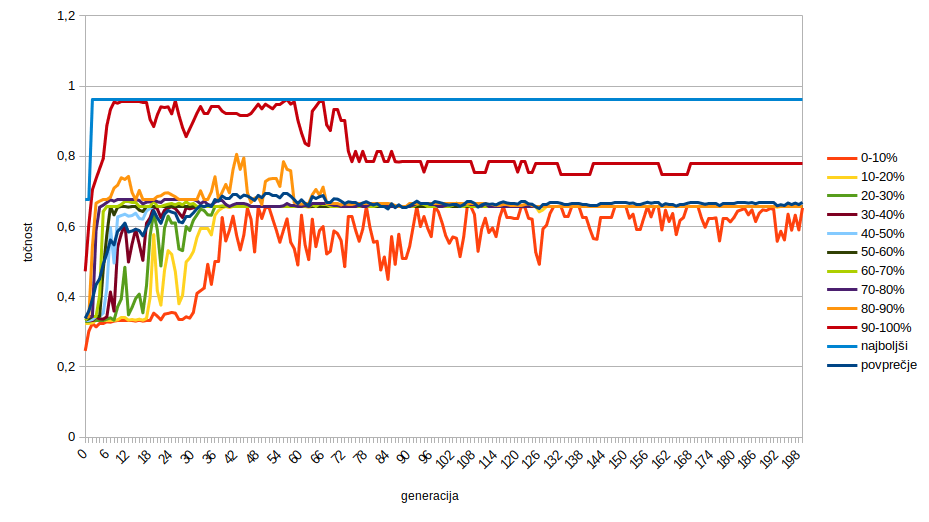
\includegraphics[width=13cm]{iris/1/acc}
    \end{center}
    \caption{Graf točnosti populacije najboljšega agenta prvega nabora skozi generacije.}
    \label{fig:iris_acc_1}
\end{figure}

\begin{figure}[H]
    \begin{center}
        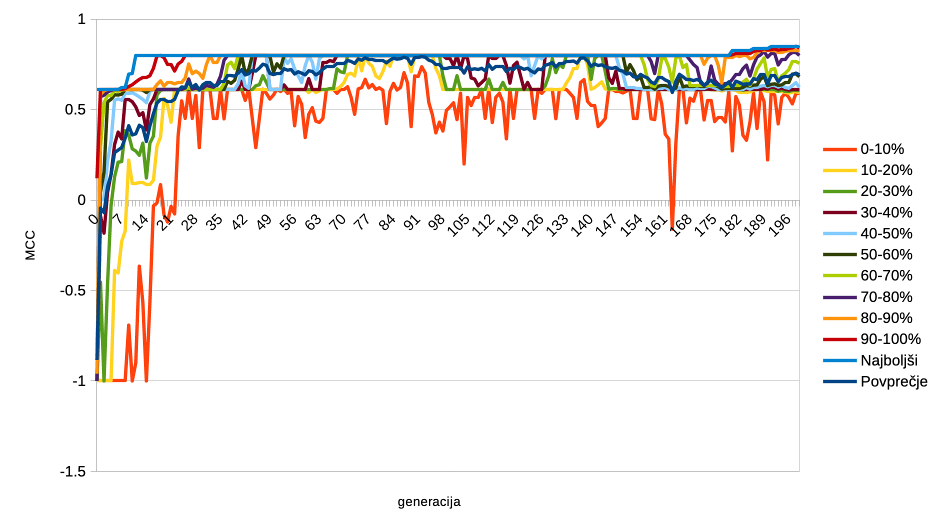
\includegraphics[width=13cm]{iris/1/mcc}
    \end{center}
    \caption{Graf MKK populacije najboljšega agenta prvega nabora skozi generacije.}
    \label{fig:iris_mcc_1}
\end{figure}

\begin{figure}[H]
    \begin{center}
        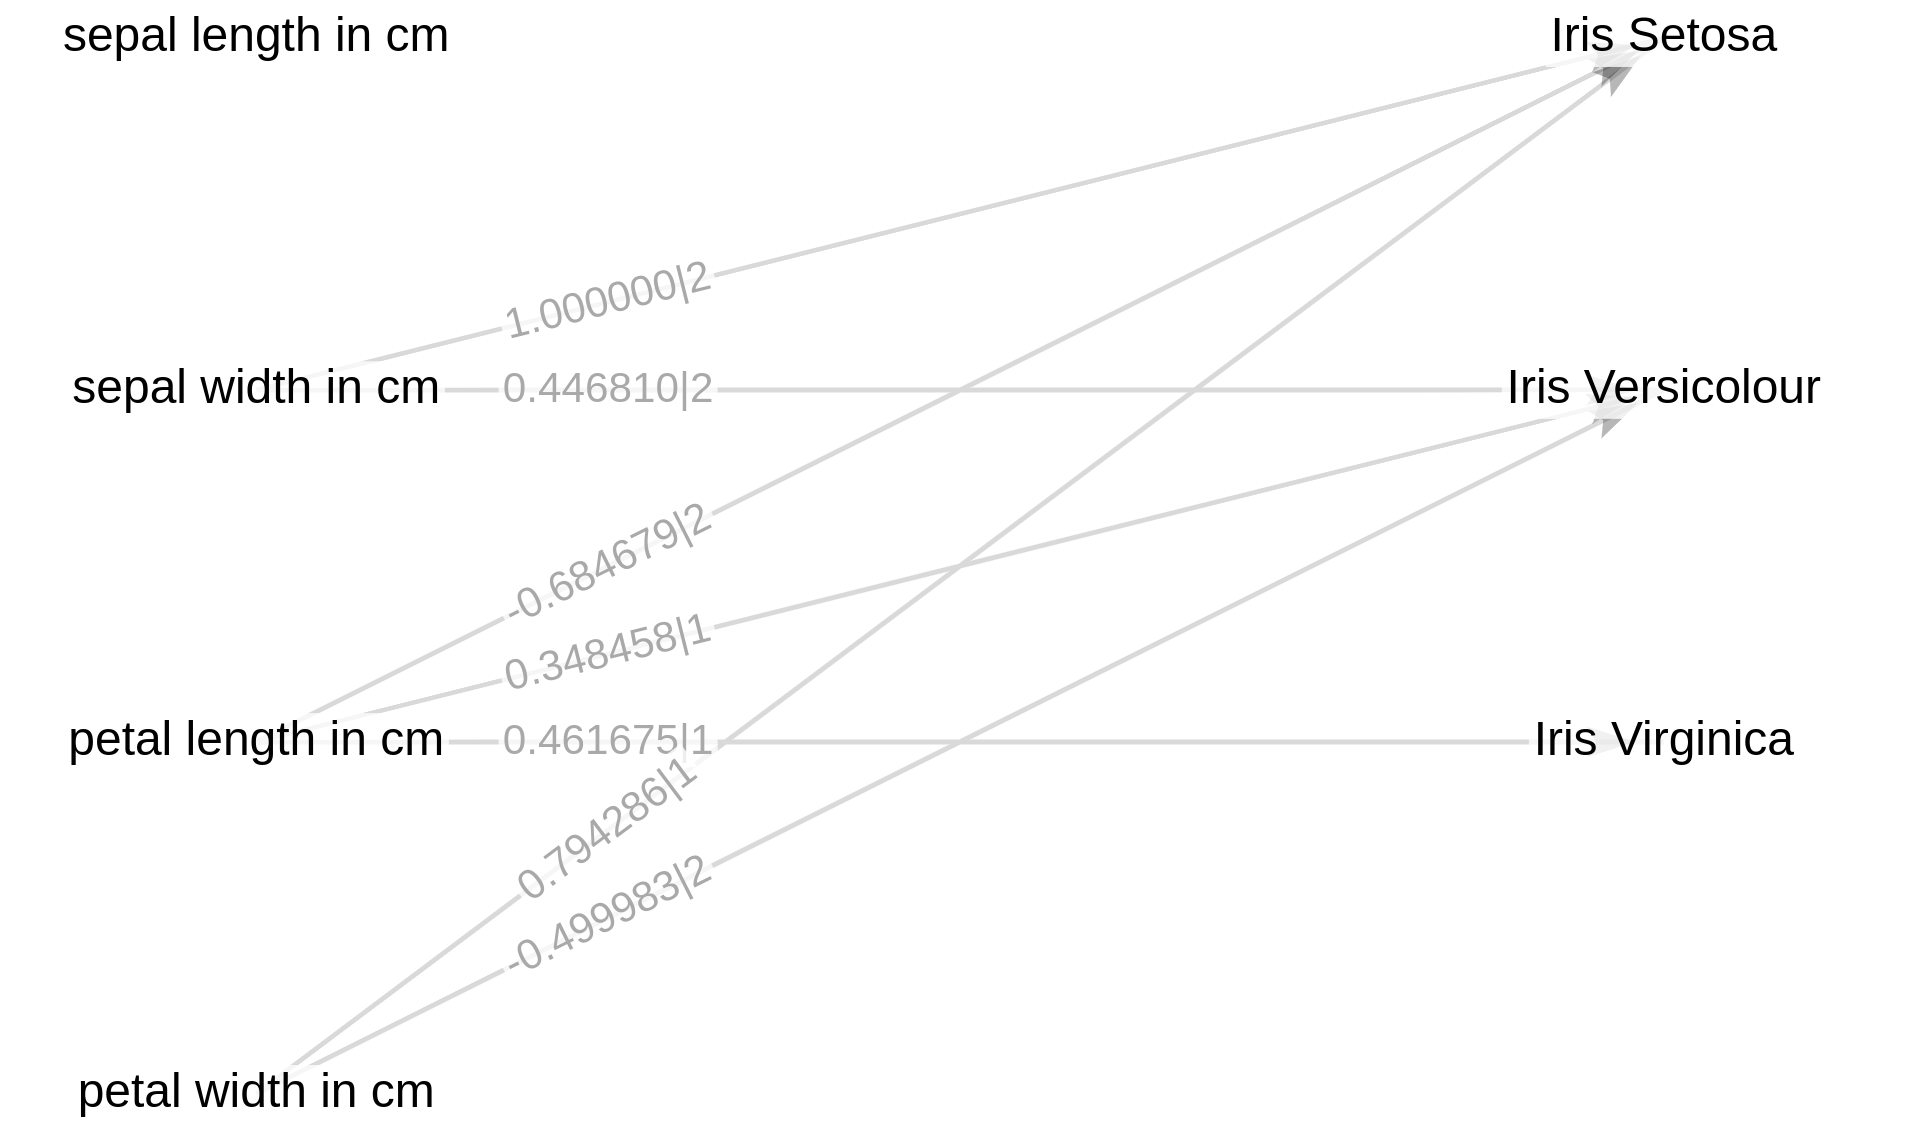
\includegraphics[width=13cm]{iris/1/acc_g}
    \end{center}
    \caption{Vizualizacija najbolj točnega agenta prvega nabora. Vsebuje 5 povezav.}
    \label{fig:iris_acc_1_g}
\end{figure}

\begin{figure}[H]
    \begin{center}
        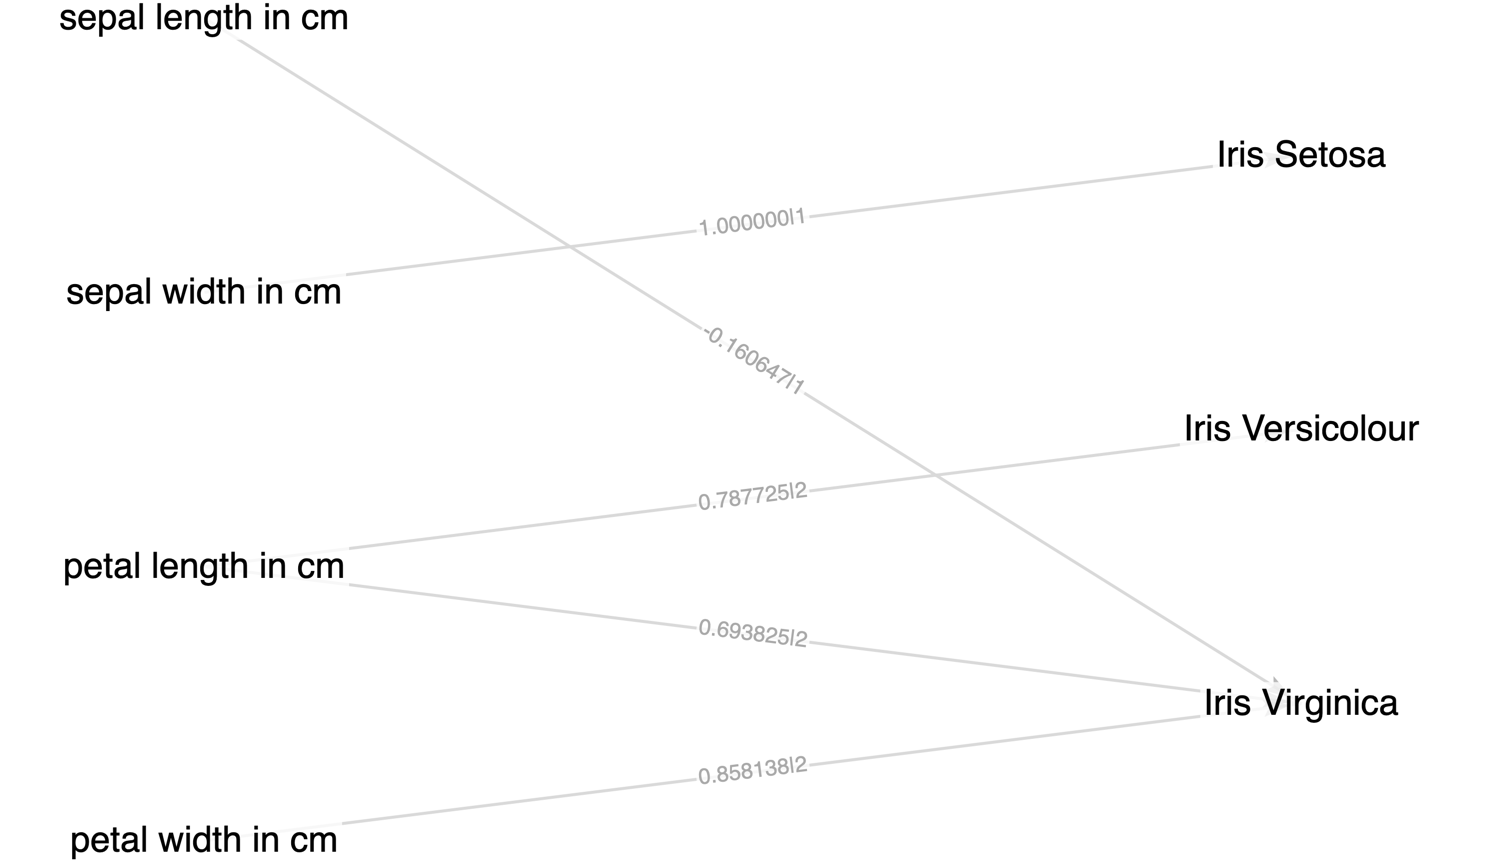
\includegraphics[width=13cm]{iris/1/mcc_g}
    \end{center}
    \caption{Vizualizacija agenta z največjim MKK prvega nabora. Vsebuje 6 povezav.}
    \label{fig:iris_mcc_1_g}
\end{figure}

\newpage

\subsection{Drugi nabor}\label{subsec:dodatek-iris-drugi-nabor}
%%"/home/jure/CLionProjects/Neuroevolution/datasets/iris/iris.data" 150 10 20 2 true 0.1 75 true -0.00001 200 ACC
\begin{table}[H]
    \begin{center}
        \begin{tabular}{|| c | c c || c c ||}
            \hline
            \multirow{2}{*}{št. zagona} & \multicolumn{2}{c||}{točnost najboljšega agenta} & \multicolumn{2}{c||}{MKK najboljšega agenta} \\ \cline{2-5}
            & učna   & testna          & učna  & testna                  \\
            \hline
            1         & 95.2\% & \textbf{97.8\%} & 0.986 & 0.901                   \\
            \hline
            2         & 96.2\% & 95.6\%          & 0.958 & 0.906                   \\
            \hline
            3         & 85.7\% & 93.3\%          & 0.958 & \textbf{0.967 (97.8\%)} \\
            \hline
            4         & 96.2\% & 93.3\%          & 0.986 & 0.902                   \\
            \hline
            5         & 95.2\% & 95.6\%          & 0.945 & 0.906                   \\
            \hline
            povprečje & 93.7\% & 94.7\%          & 0.967 & 0.916                   \\
            \hline
            $\sigma$  & 0.040  & 0.017           & 0.017 & 0.025                   \\
            \hline
        \end{tabular}
    \end{center}
    \caption{Rezultat drugega nabora parametrov.}
    \label{tab:iris_result_2}
\end{table}

\begin{table}[H]
    \centering
    \begin{tabular}{||rcccc||}
        \hline
        razred           & Iris Setosa & Iris Versicolour & Iris Virginica & vsota \\ \hline
        ris Setosa       & 15          & 0                & 0              & 15    \\ \hline
        Iris Versicolour & 0           & 15               & 0              & 15    \\ \hline
        Iris Virginica   & 0           & 1                & 14             & 15    \\ \hline
        vsota            & 15          & 16               & 14             & 45    \\ \hline
    \end{tabular}
    \caption{Matrika zmot najbolj točnega agenta drugega nabora.}
    \label{tab:iris_acc_2}
\end{table}

\begin{table}[H]
    \centering
    \begin{tabular}{||rcccc||}
        \hline
        razred           & Iris Setosa & Iris Versicolour & Iris Virginica & vsota \\ \hline
        ris Setosa       & 15          & 0                & 0              & 15    \\ \hline
        Iris Versicolour & 0           & 14               & 1              & 15    \\ \hline
        Iris Virginica   & 0           & 0                & 15             & 15    \\ \hline
        vsota            & 15          & 14               & 16             & 45    \\ \hline
    \end{tabular}
    \caption{Matrika zmot agenta z največjim MKK drugega nabora.}
    \label{tab:iris_mcc_2}
\end{table}

\begin{figure}[H]
    \begin{center}
        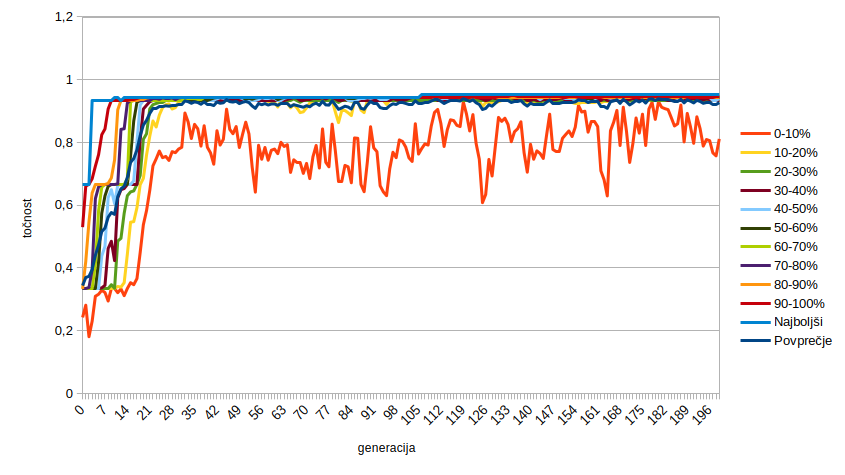
\includegraphics[width=13cm]{iris/2/acc}
    \end{center}
    \caption{Graf točnosti populacije najboljšega agenta drugega nabora skozi generacije.}
    \label{fig:iris_acc_2}
\end{figure}

\begin{figure}[H]
    \begin{center}
        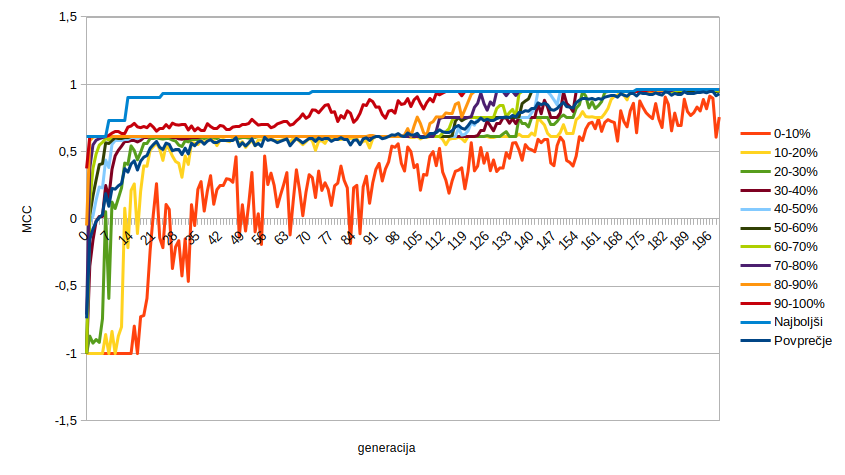
\includegraphics[width=13cm]{iris/2/mcc}
    \end{center}
    \caption{Graf MKK populacije najboljšega agenta drugega nabora skozi generacije.}
    \label{fig:iris_mcc_2}
\end{figure}

\begin{figure}[H]
    \begin{center}
        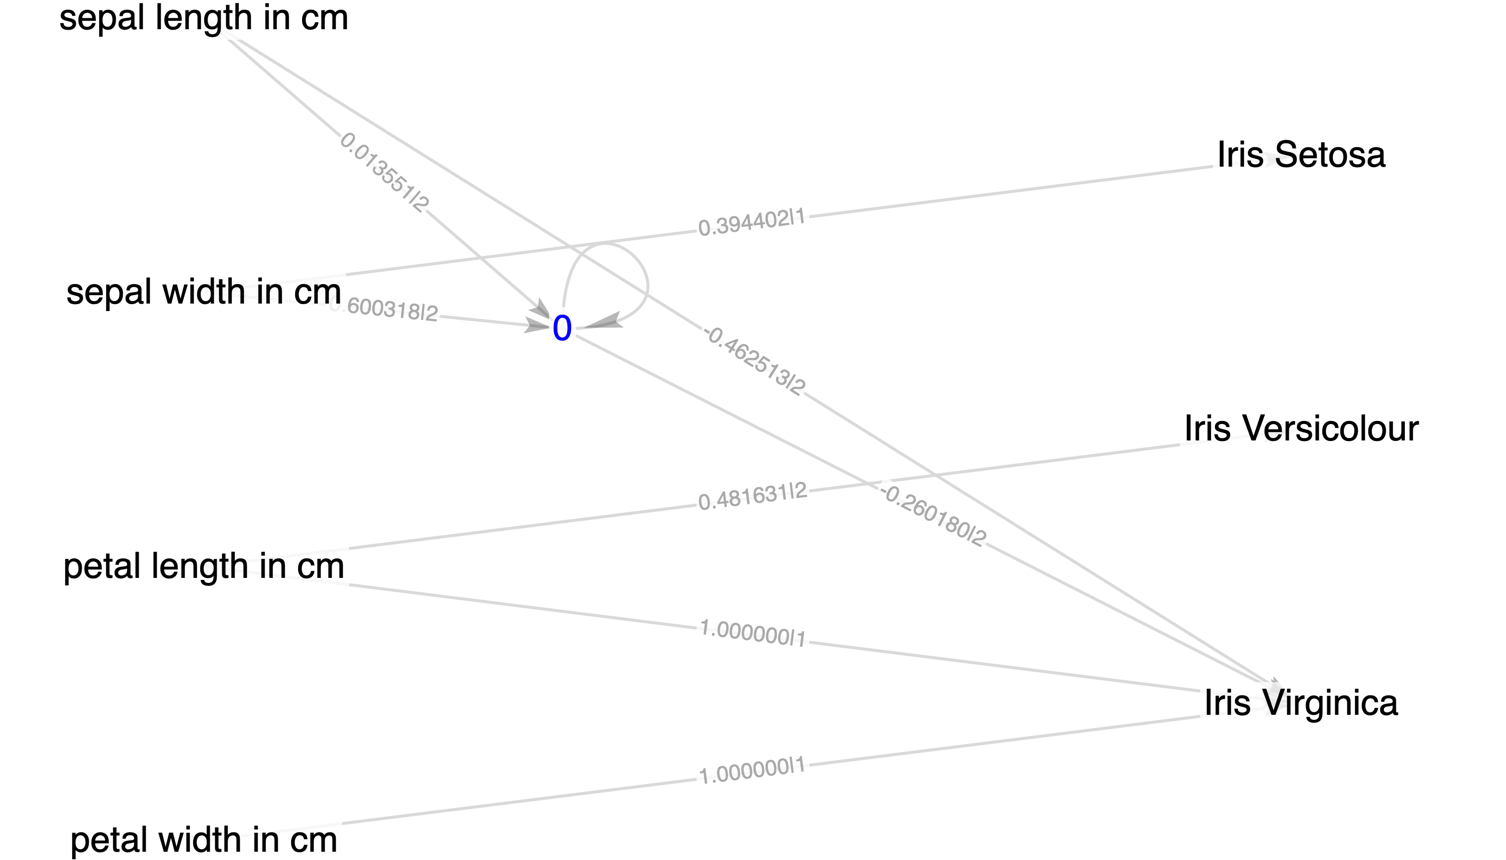
\includegraphics[width=13cm]{iris/2/acc_g}
    \end{center}
    \caption{Vizualizacija najbolj točnega agenta drugega nabora. Vsebuje 2 vmesni vozlišči in 8 povezav.}
    \label{fig:iris_acc_2_g}
\end{figure}

\begin{figure}[H]
    \begin{center}
        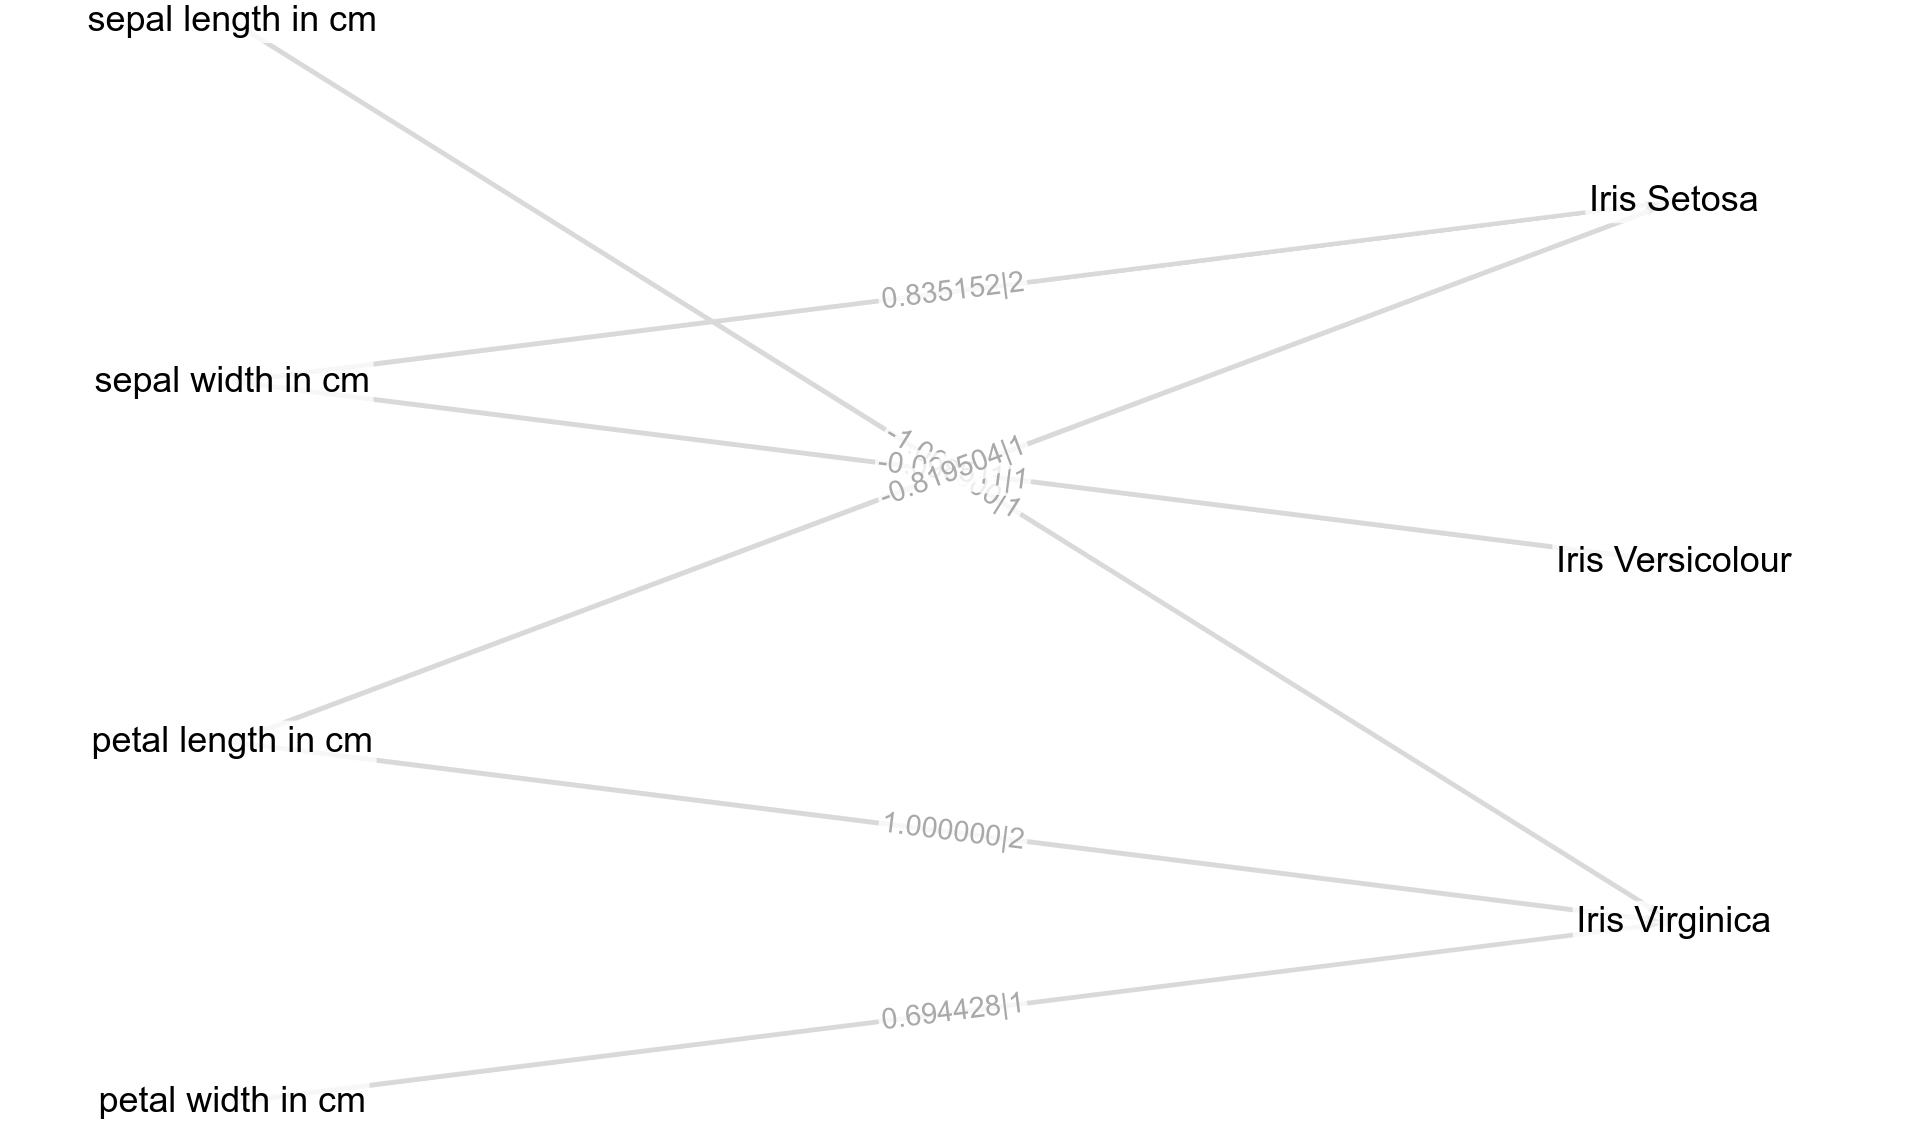
\includegraphics[width=13cm]{iris/2/mcc_g}
    \end{center}
    \caption{Vizualizacija agenta z največjim MKK drugega nabora. Vsebuje 6 povezav.}
    \label{fig:iris_mcc_2_g}
\end{figure}

\subsection{Tretji nabor}\label{subsec:dodatek-iris-tretji-nabor}
%%"/home/jure/CLionProjects/Neuroevolution/datasets/iris/iris.data" 200 15 30 3 true 0.1 100 true -0.00001 300 ACC
\begin{table}[H]
    \begin{center}
        \begin{tabular}{|| c | c c || c c ||}
            \hline
            \multirow{2}{*}{št. zagona} & \multicolumn{2}{c||}{točnost najboljšega agenta} & \multicolumn{2}{c||}{MKK najboljšega agenta} \\ \cline{2-5}
            & učna   & testna          & učna  & testna                  \\
            \hline
            1         & 97.1\% & 95.6\%          & 0.958 & 0.849                   \\
            \hline
            2         & 89.5\% & 75.6\%          & 0.945 & \textbf{0.936 (95.6\%)} \\
            \hline
            3         & 97.1\% & 93.3\%          & 0.972 & 0.834                   \\
            \hline
            4         & 95.2\% & \textbf{97.8\%} & 0.972 & 0.934                   \\
            \hline
            5         & 97.1\% & 97.8\%          & 0.972 & 0.936                   \\
            \hline
            povprečje & 95.2\% & 92.0\%          & 0.964 & 0.898                   \\
            \hline
            $\sigma$  & 0.029  & 0.084           & 0.011 & 0.046                   \\
            \hline
        \end{tabular}
    \end{center}
    \caption{Rezultat tretjega nabora parametrov.}
    \label{tab:iris_result_3}
\end{table}

\begin{table}[H]
    \centering
    \begin{tabular}{||rcccc||}
        \hline
        razred           & Iris Setosa & Iris Versicolour & Iris Virginica & vsota \\ \hline
        ris Setosa       & 14          & 1                & 0              & 15    \\ \hline
        Iris Versicolour & 0           & 15               & 0              & 15    \\ \hline
        Iris Virginica   & 0           & 0                & 15             & 15    \\ \hline
        vsota            & 14          & 15               & 15             & 45    \\ \hline
    \end{tabular}
    \caption{Matrika zmot najbolj točnega agenta tretjega nabora.}
    \label{tab:iris_acc_3}
\end{table}

\begin{table}[H]
    \centering
    \begin{tabular}{||rcccc||}
        \hline
        razred           & Iris Setosa & Iris Versicolour & Iris Virginica & vsota \\ \hline
        ris Setosa       & 15          & 0                & 0              & 15    \\ \hline
        Iris Versicolour & 0           & 13               & 2              & 15    \\ \hline
        Iris Virginica   & 0           & 0                & 15             & 15    \\ \hline
        vsota            & 15          & 13               & 17             & 45    \\ \hline
    \end{tabular}
    \caption{Matrika zmot agenta z največjim MKK tretjega nabora.}
    \label{tab:iris_mcc_3}
\end{table}

\begin{figure}[H]
    \begin{center}
        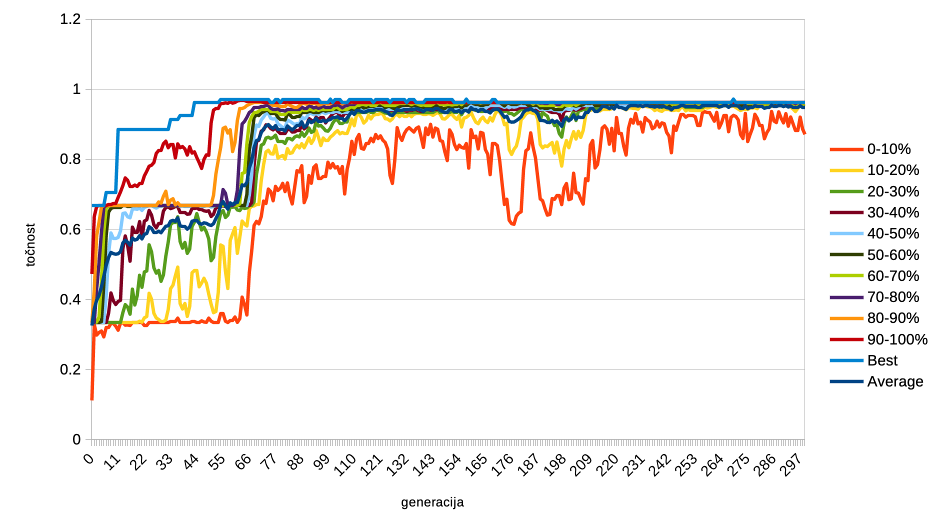
\includegraphics[width=13cm]{iris/3/acc}
    \end{center}
    \caption{Graf točnosti populacije najboljšega agenta tretjega nabora skozi generacije.}
    \label{fig:iris_acc_3}
\end{figure}

\begin{figure}[H]
    \begin{center}
        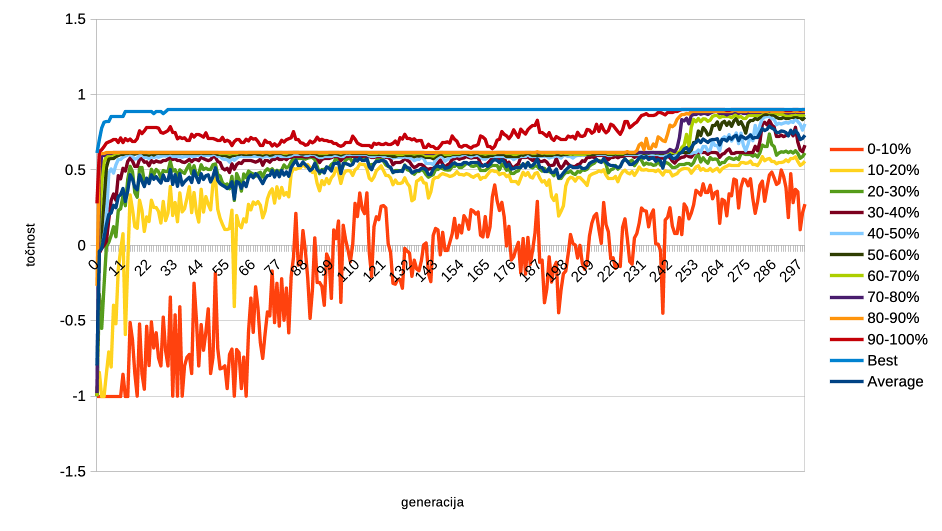
\includegraphics[width=13cm]{iris/3/mcc}
    \end{center}
    \caption{Graf MKK populacije najboljšega agenta tretjega nabora skozi generacije.}
    \label{fig:iris_mcc_3}
\end{figure}

\begin{figure}[H]
    \begin{center}
        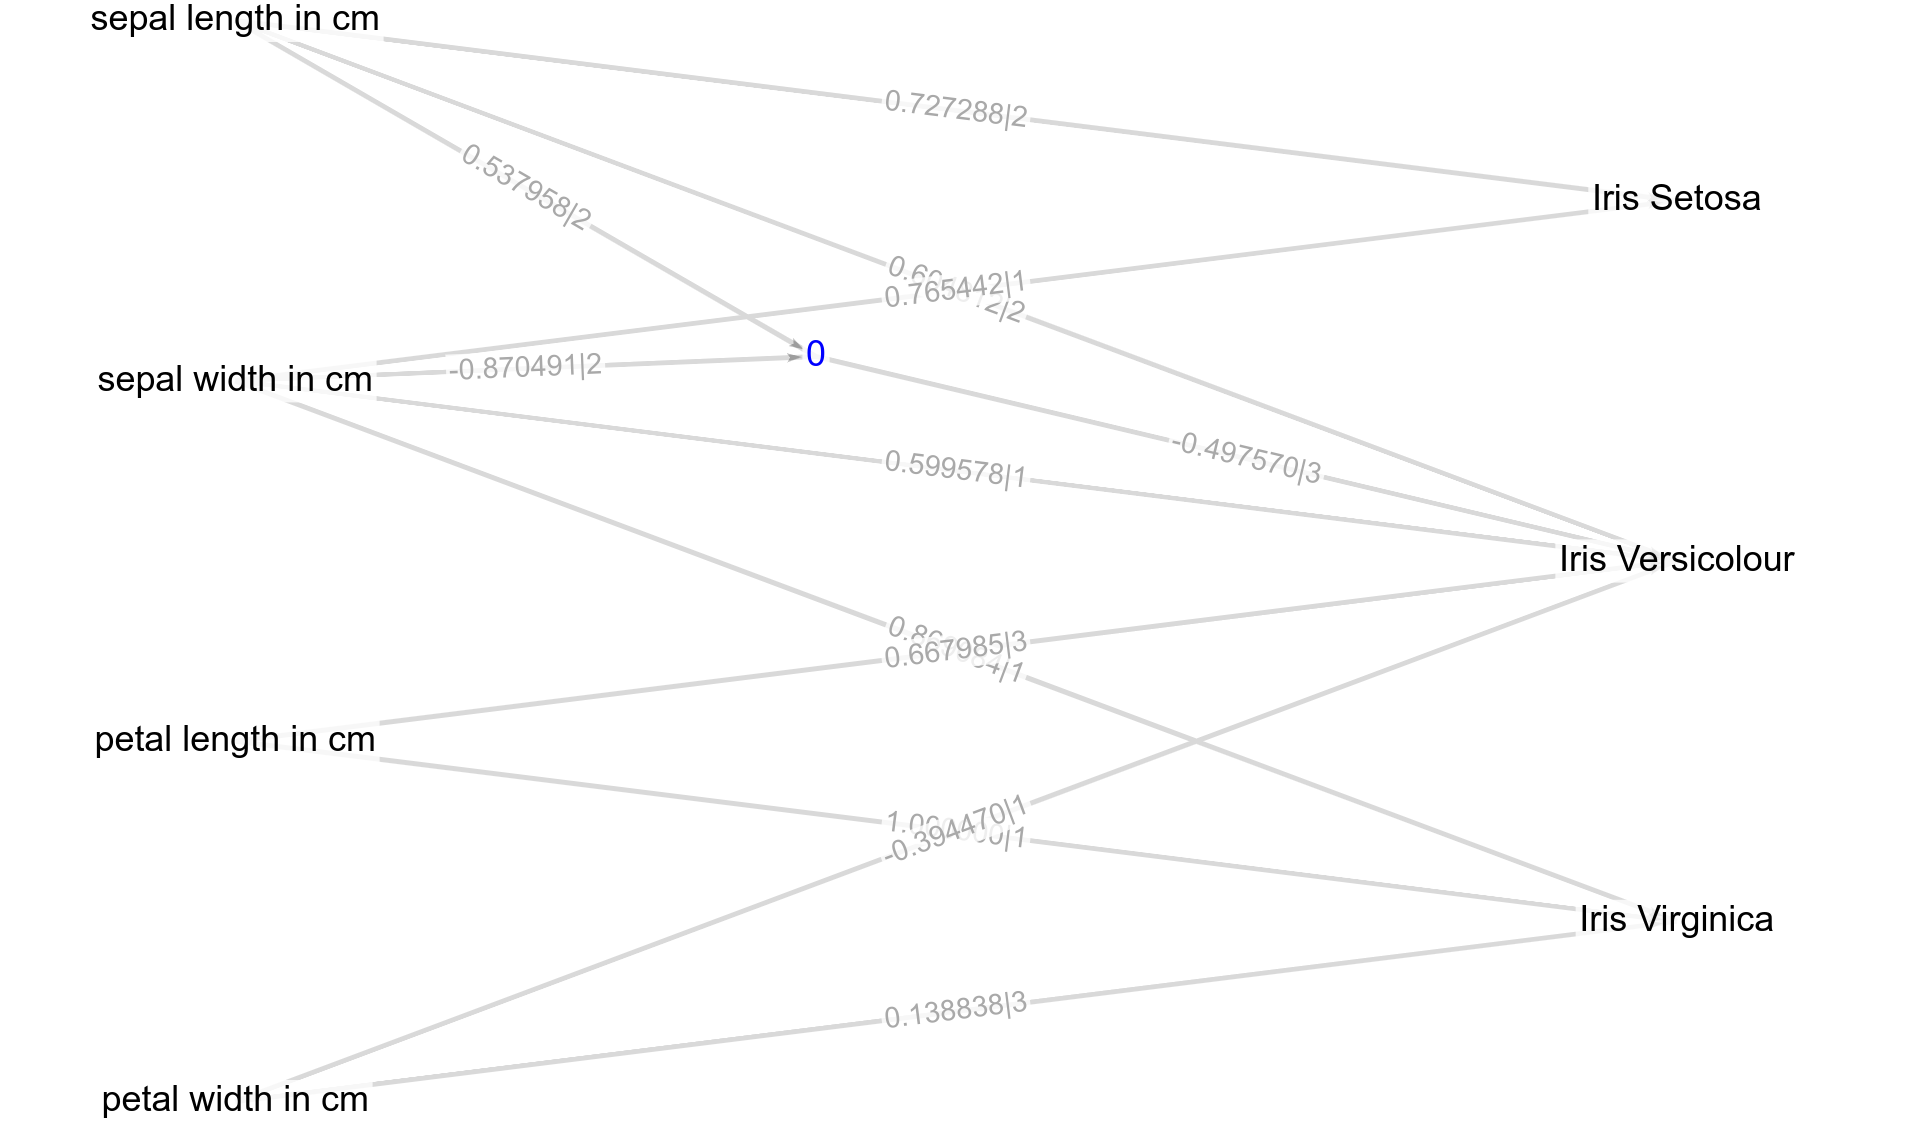
\includegraphics[width=13cm]{iris/3/acc_g}
    \end{center}
    \caption{Vizualizacija najbolj točnega agenta tretjega nabora. Vsebuje 1 vmesno vozlišče in 12 povezav.}
    \label{fig:iris_acc_3_g}
\end{figure}

\begin{figure}[H]
    \begin{center}
        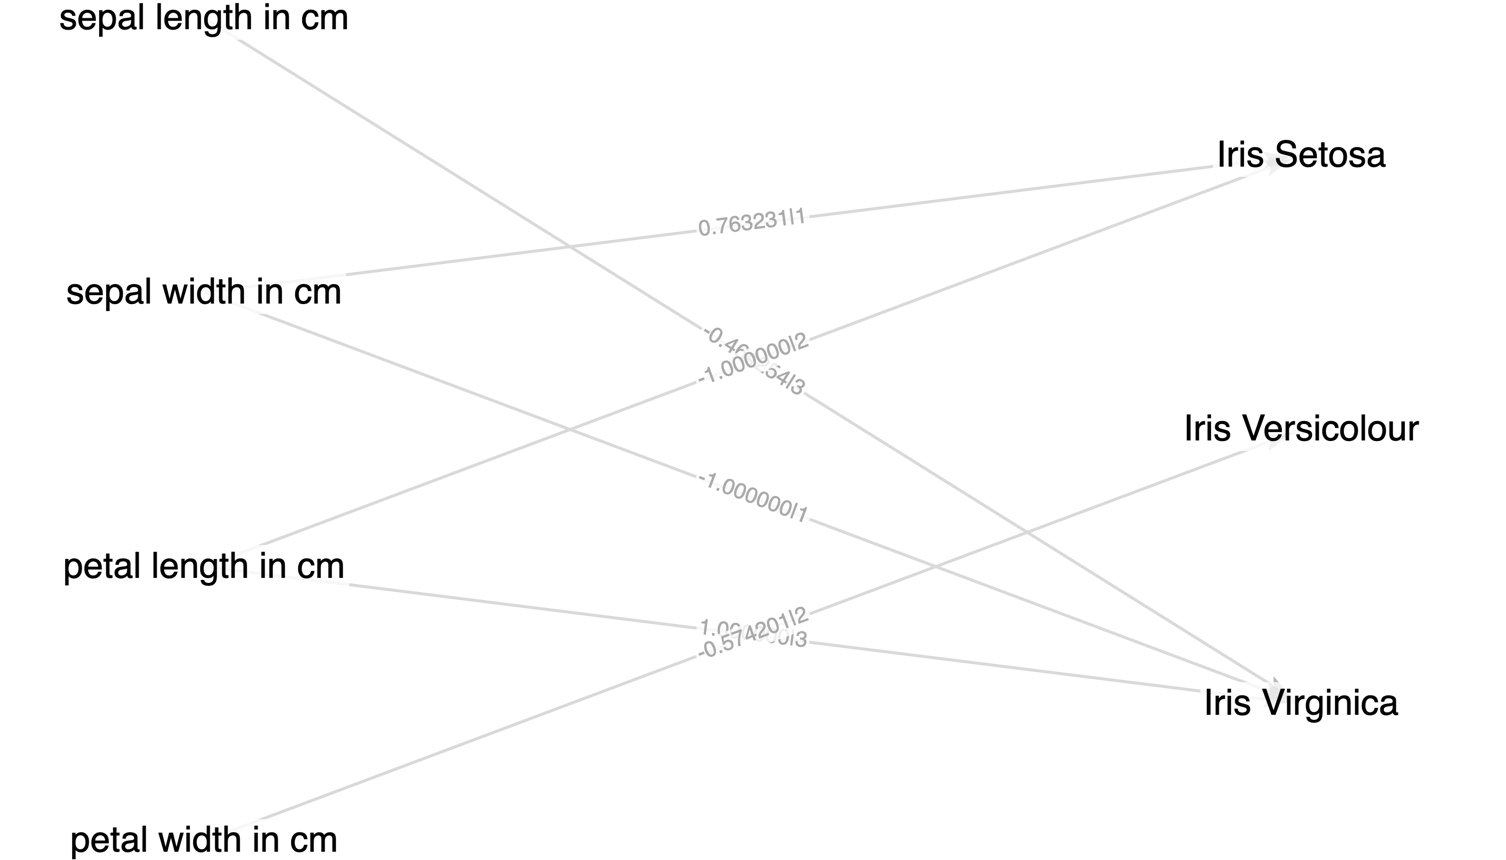
\includegraphics[width=13cm]{iris/3/mcc_g}
    \end{center}
    \caption{Vizualizacija agenta z največjim MKK drugega nabora. Vsebuje 1 vmesno vozlišče in 9 povezav.}
    \label{fig:iris_mcc_3_g}
\end{figure}

\section{Wine}\label{sec:dodatek-wine-test}
%% arrowLength=20
%% linkWidth=2
%% input fy=50*node.pos
%% output fx=700
%% output fy=150*node.pos+120
%% MAX_FONT_SIZE=12
\begin{table}[H]
    \begin{center}
        \begin{tabular}{||l c c c||}
            \hline
            & 1      & 2      & 3 \\ [0.5ex]
            \hline
            velikost populacije               & 200    & 250    & 350    \\
            \hline
            največje število globokih vozlišč & 15     & 20     & 25     \\
            \hline
            največje število povezav          & 30     & 50     & 75     \\
            \hline
            največje število prečkanj         & 2      & 3      & 4      \\
            \hline
            delež mutiranih potomcev          & 10\%   & 10\%   & 10\%   \\
            \hline
            prispevek vozlišč                 & -0.001 & -0.001 & -0.001 \\
            \hline
            prispevek povezav                 & -0.001 & -0.001 & -0.001 \\
            \hline
            število generacij                 & 300    & 350    & 450    \\
            \hline
        \end{tabular}
    \end{center}
    \caption{Nabori inicializacijskih parametrov poganjanja na množici Wine.}
    \label{tab:param_wine}
\end{table}

\subsection{Prvi nabor}\label{subsec:dodatek-wine-prvi-nabor}
%%"/home/jure/CLionProjects/Neuroevolution/datasets/wine/wine.data" 200 15 30 2 true 0.1 100 true -0.001 -0.001 300 ACC
\begin{table}[H]
    \begin{center}
        \begin{tabular}{|| c | c c || c c ||}
            \hline
            \multirow{2}{*}{št. zagona} & \multicolumn{2}{c||}{točnost najboljšega agenta} & \multicolumn{2}{c||}{MCC najboljšega agenta} \\ \cline{2-5}
            & učna   & testna          & učna  & testna                  \\
            \hline
            1        & 92.0\% & 75.5\%          & 0.868 & \textbf{0.918 (94.3\%)} \\
            \hline
            2        & 94.4\% & 92.5\%          & 0.808 & 0.843                   \\
            \hline
            3        & 92.0\% & 92.5\%          & 0.818 & 0.779                   \\
            \hline
            4        & 96.8\% & \textbf{94.3\%} & 0.820 & 0.677                   \\
            \hline
            5        & 84.8\% & 75.5\%          & 0.904 & 0.830                   \\
            \hline
            $\sigma$ & 0.040  & 0.086           & 0.037 & 0.08                    \\
            \hline
        \end{tabular}
    \end{center}
    \caption{Rezultat prvega nabora parametrov.}
    \label{tab:wine_result_1}
\end{table}

\begin{table}[H]
    \centering
    \begin{tabular}{||rcccc||}
        \hline
        razred  & Class 1 & Class 2 & Class 3 & vsota \\ \hline
        Class 1 & 17      & 1       & 0       & 18    \\ \hline
        Class 2 & 2       & 19      & 0       & 21    \\ \hline
        Class 3 & 0       & 0       & 14      & 14    \\ \hline
        vsota   & 19      & 20      & 14      & 53    \\ \hline
    \end{tabular}
    \caption{Matrika zmot najbolj točnega agenta prvega nabora.}
    \label{tab:wine_acc_1}
\end{table}

\begin{table}[H]
    \centering
    \begin{tabular}{||rcccc||}
        \hline
        razred  & Class 1 & Class 2 & Class 3 & vsota \\ \hline
        Class 1 & 18      & 0       & 0       & 18    \\ \hline
        Class 2 & 2       & 18      & 1       & 21    \\ \hline
        Class 3 & 0       & 0       & 14      & 14    \\ \hline
        vsota   & 20      & 18      & 15      & 53    \\ \hline
    \end{tabular}
    \caption{Matrika zmot agenta z največjim MCC prvega nabora.}
    \label{tab:wine_mcc_1}
\end{table}

\begin{figure}[H]
    \begin{center}
        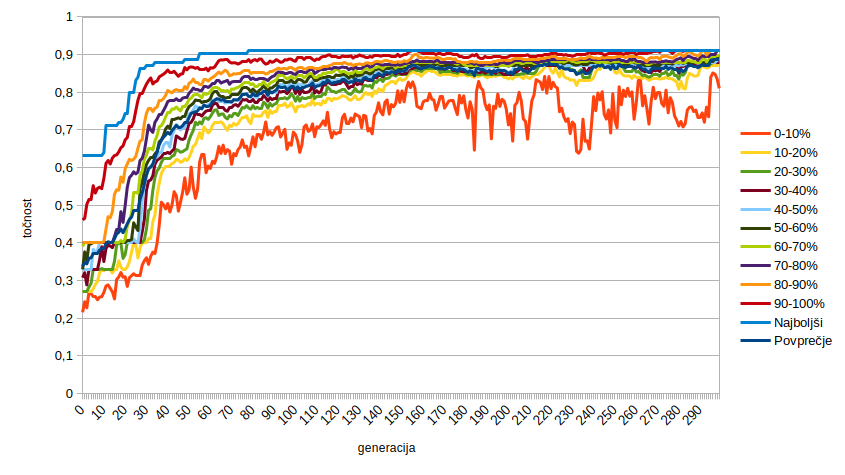
\includegraphics[width=13cm]{wine/1/acc}
    \end{center}
    \caption{Graf točnosti populacije najboljšega agenta prvega nabora skozi generacije.}
    \label{fig:wine_acc_1}
\end{figure}

\begin{figure}[H]
    \begin{center}
        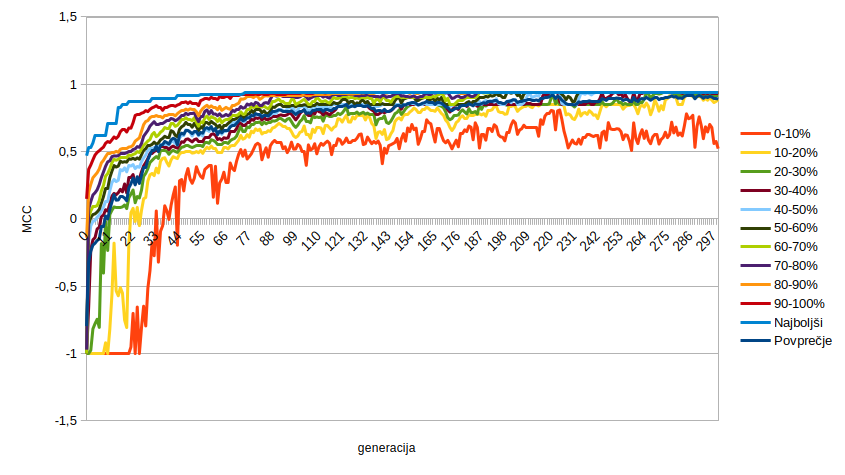
\includegraphics[width=13cm]{wine/1/mcc}
    \end{center}
    \caption{Graf MCC populacije najboljšega agenta prvega nabora skozi generacije.}
    \label{fig:wine_mcc_1}
\end{figure}

\begin{figure}[H]
    \begin{center}
        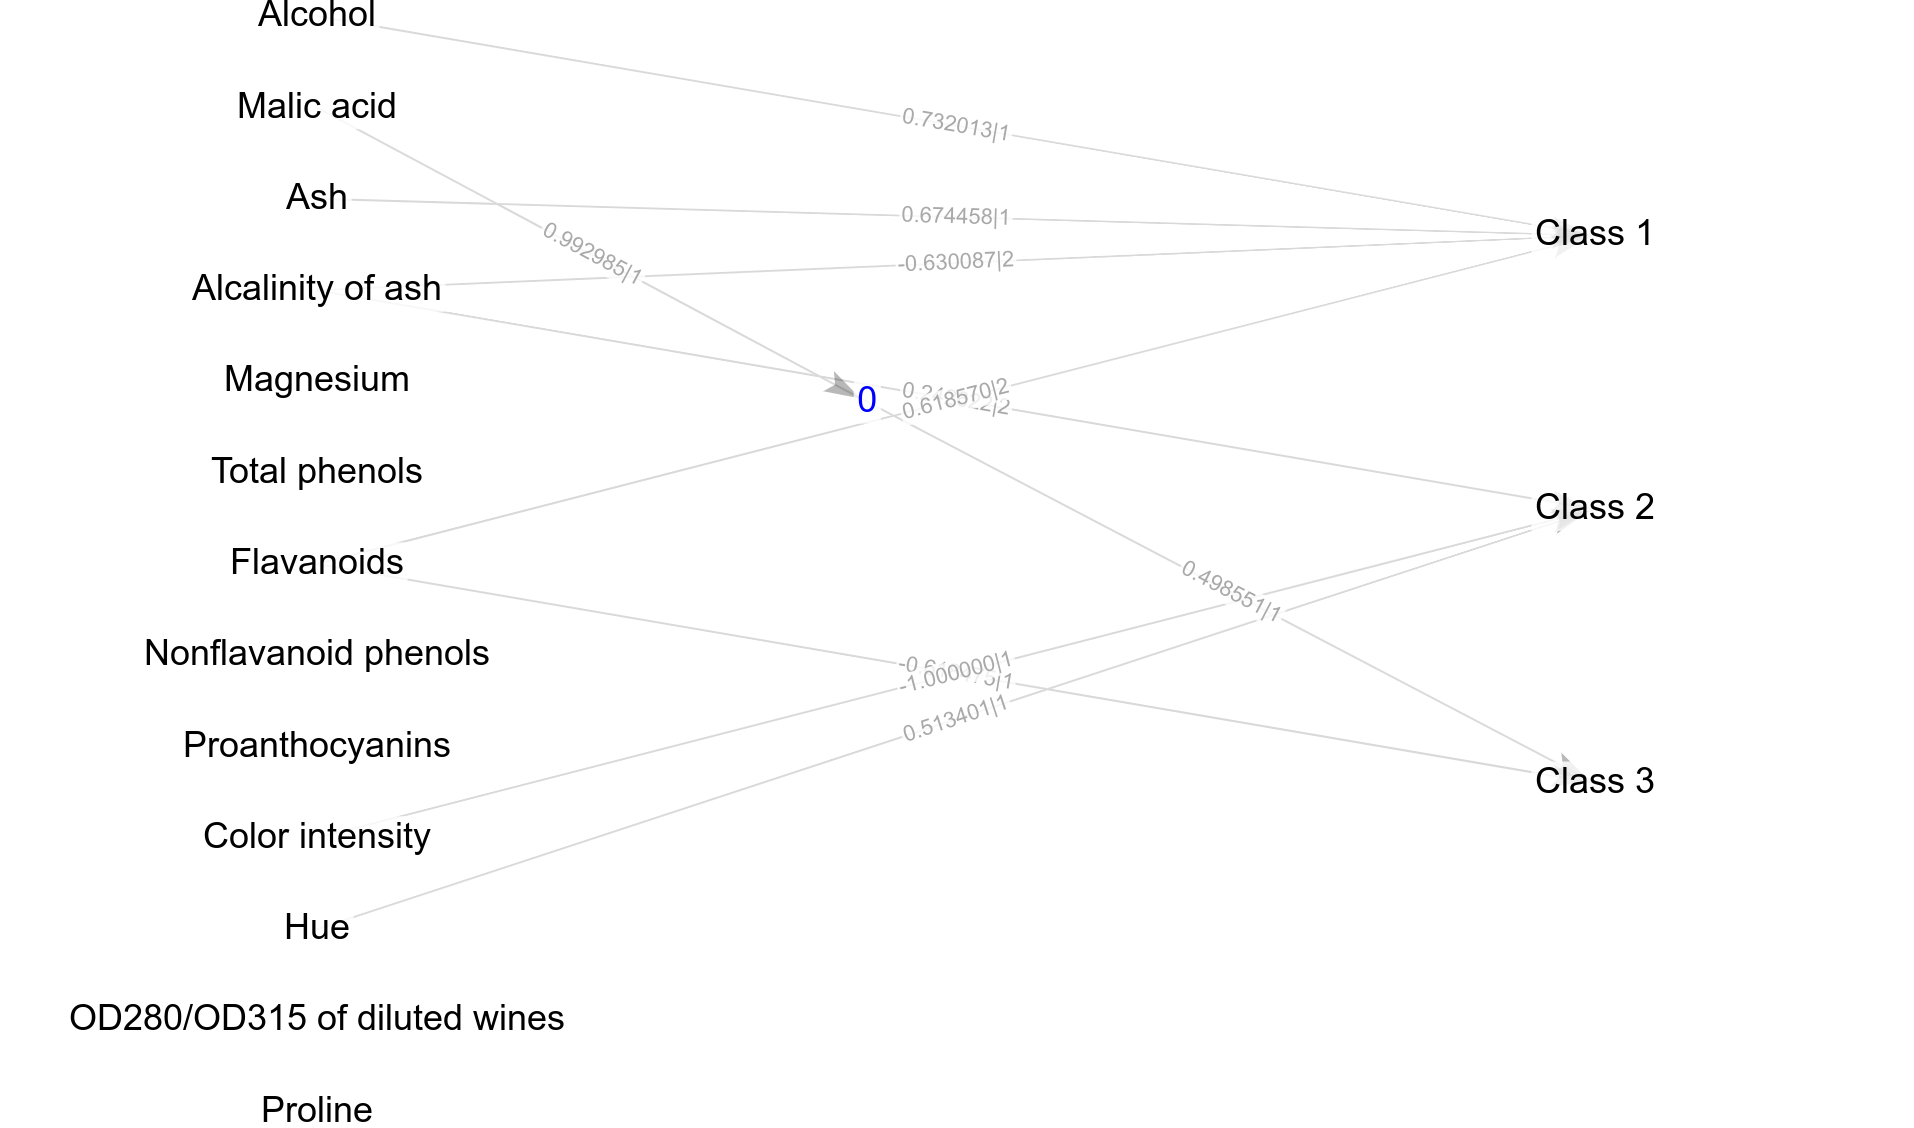
\includegraphics[width=13cm]{wine/1/acc_g}
    \end{center}
    \caption{Vizualizacija najbolj točnega agenta prvega nabora. Vsebuje 1 globoko vozlišče in 9 povezav.}
    \label{fig:wine_acc_1_g}
\end{figure}

\begin{figure}[H]
    \begin{center}
        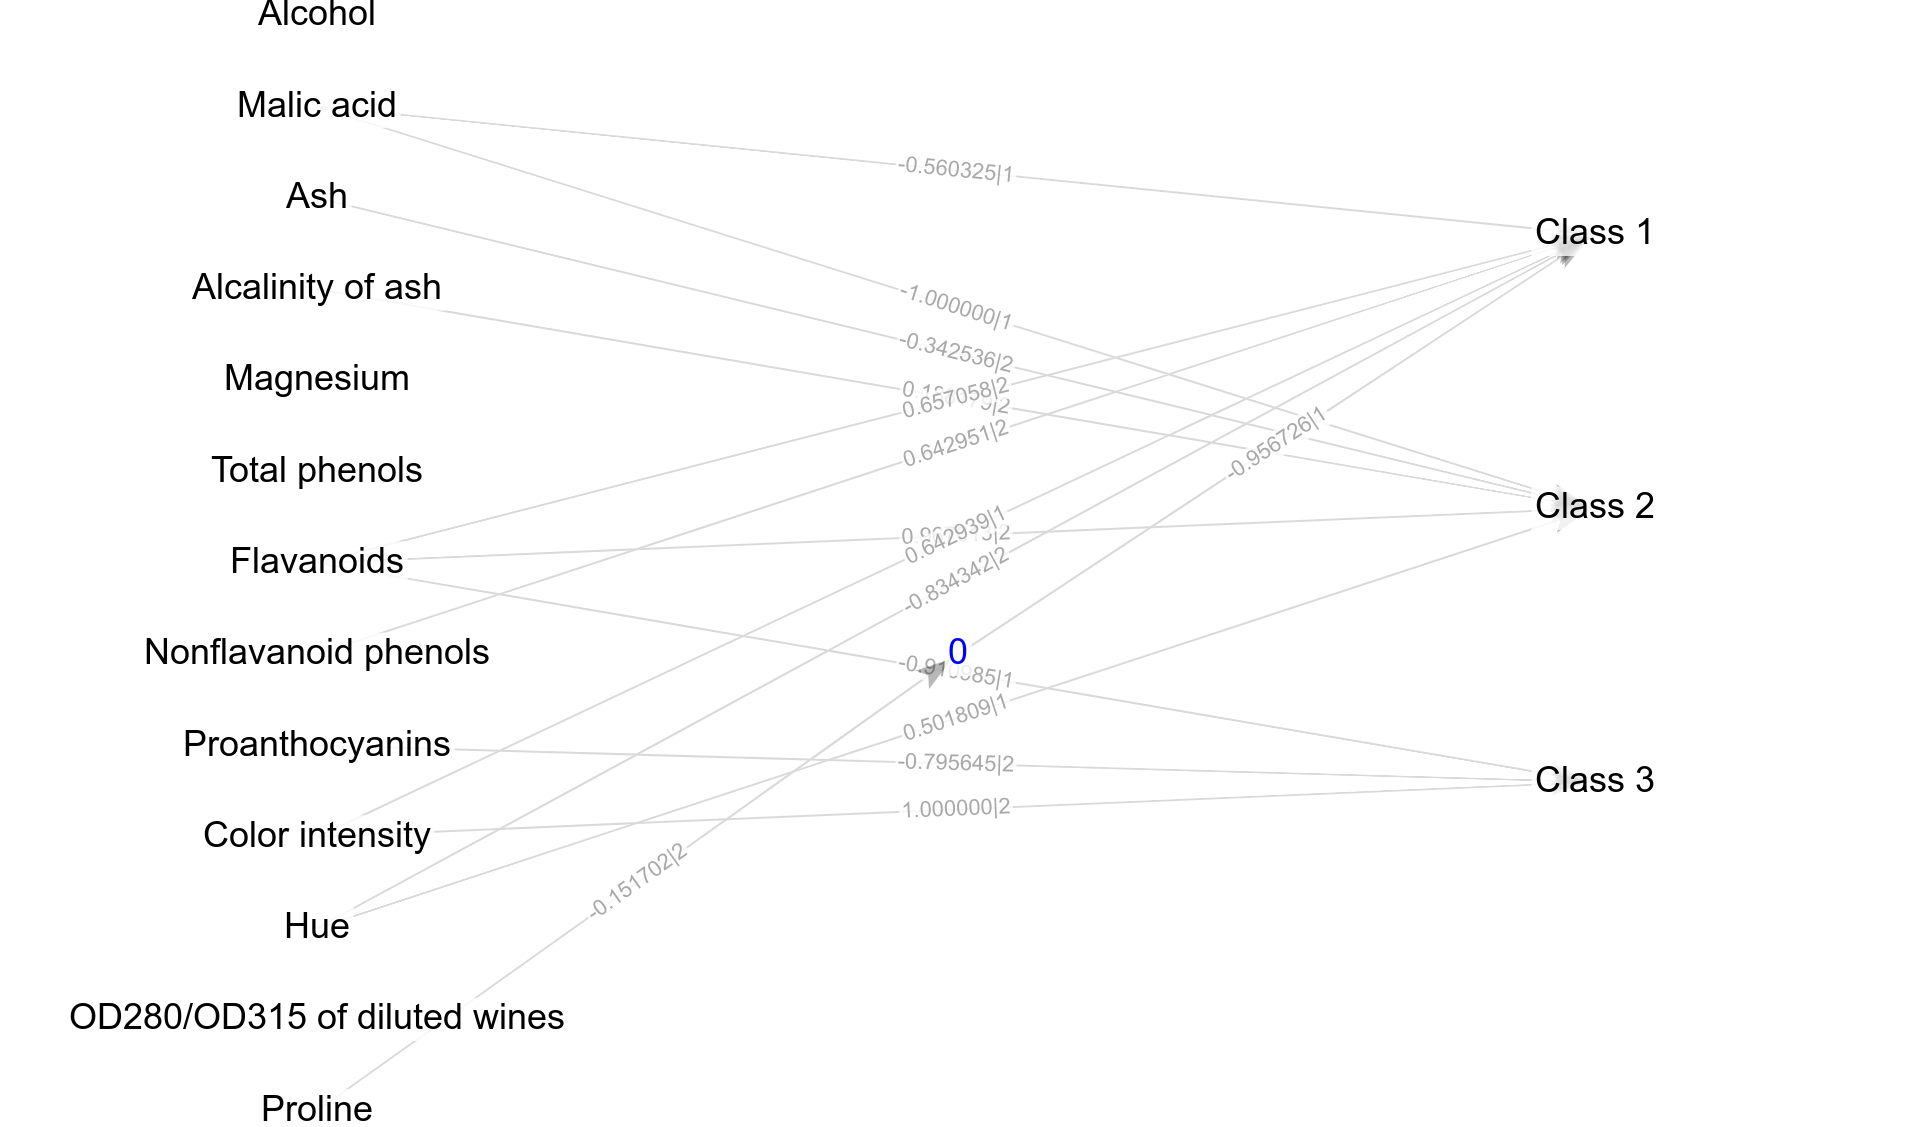
\includegraphics[width=13cm]{wine/1/mcc_g}
    \end{center}
    \caption{Vizualizacija agenta z največjim MCC prvega nabora. Vsebuje 6 povezav.}
    \label{fig:wine_mcc_1_g}
\end{figure}

\subsection{Drugi nabor}\label{subsec:dodatek-wine-drugi-nabor}
%%"/home/jure/CLionProjects/Neuroevolution/datasets/iris/iris.data" 250 20 50 3 true 0.1 100 true -0.001 -0.001 350 ACC
\begin{table}[H]
    \begin{center}
        \begin{tabular}{|| c | c c || c c ||}
            \hline
            \multirow{2}{*}{št. zagona} & \multicolumn{2}{c||}{točnost najboljšega agenta} & \multicolumn{2}{c||}{MCC najboljšega agenta} \\ \cline{2-5}
            & učna   & testna          & učna  & testna                  \\
            \hline
            1        & 83.2\% & 81.1\%          & 0.845 & 0.610                   \\
            \hline
            2        & 67.2\% & 60.4\%          & 0.867 & 0.779                   \\
            \hline
            3        & 76.8\% & 77.4\%          & 0.830 & 0.740                   \\
            \hline
            4        & 92.0\% & \textbf{96.2\%} & 0.915 & \textbf{0.915 (94.3\%)} \\
            \hline
            5        & 93.6\% & 96.2\%          & 0.892 & 0.914                   \\
            \hline
            $\sigma$ & 0.098  & 0.134           & 0.031 & 0.115                   \\
            \hline
        \end{tabular}
    \end{center}
    \caption{Rezultat drugega nabora parametrov.}
    \label{tab:wine_result_2}
\end{table}

\begin{table}[H]
    \centering
    \begin{tabular}{||rcccc||}
        \hline
        razred  & Class 1 & Class 2 & Class 3 & vsota \\ \hline
        Class 1 & 17      & 1       & 0       & 18    \\ \hline
        Class 2 & 0       & 20      & 1       & 21    \\ \hline
        Class 3 & 0       & 0       & 14      & 14    \\ \hline
        vsota   & 17      & 21      & 15      & 53    \\ \hline
    \end{tabular}
    \caption{Matrika zmot najbolj točnega agenta drugega nabora.}
    \label{tab:wine_acc_2}
\end{table}

\begin{table}[H]
    \centering
    \begin{tabular}{||rcccc||}
        \hline
        razred  & Class 1 & Class 2 & Class 3 & vsota \\ \hline
        Class 1 & 17      & 1       & 0       & 18    \\ \hline
        Class 2 & 2       & 19      & 0       & 21    \\ \hline
        Class 3 & 0       & 0       & 14      & 14    \\ \hline
        vsota   & 19      & 20      & 14      & 53    \\ \hline
    \end{tabular}
    \caption{Matrika zmot agenta z največjim MCC drugega nabora.}
    \label{tab:wine_mcc_2}
\end{table}

\begin{figure}[H]
    \begin{center}
        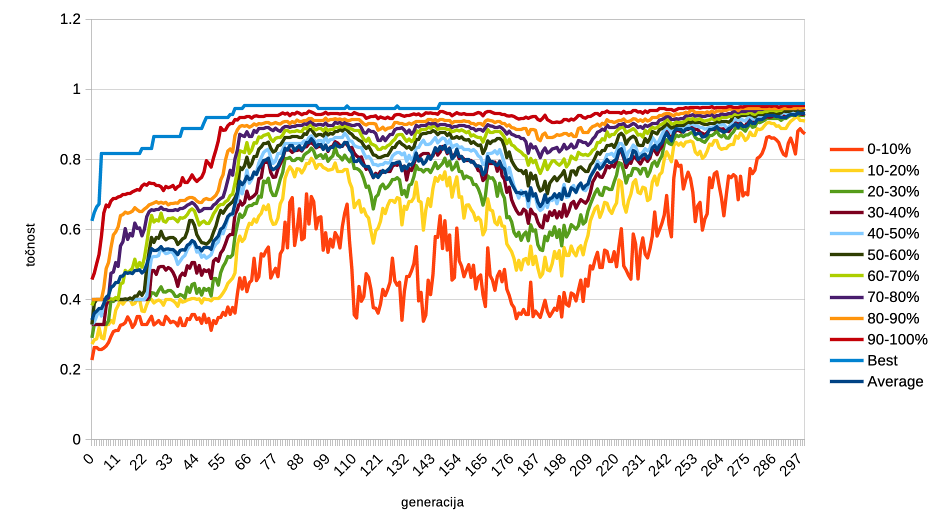
\includegraphics[width=13cm]{wine/2/acc}
    \end{center}
    \caption{Graf točnosti populacije najboljšega agenta drugega nabora skozi generacije.}
    \label{fig:wine_acc_2}
\end{figure}

\begin{figure}[H]
    \begin{center}
        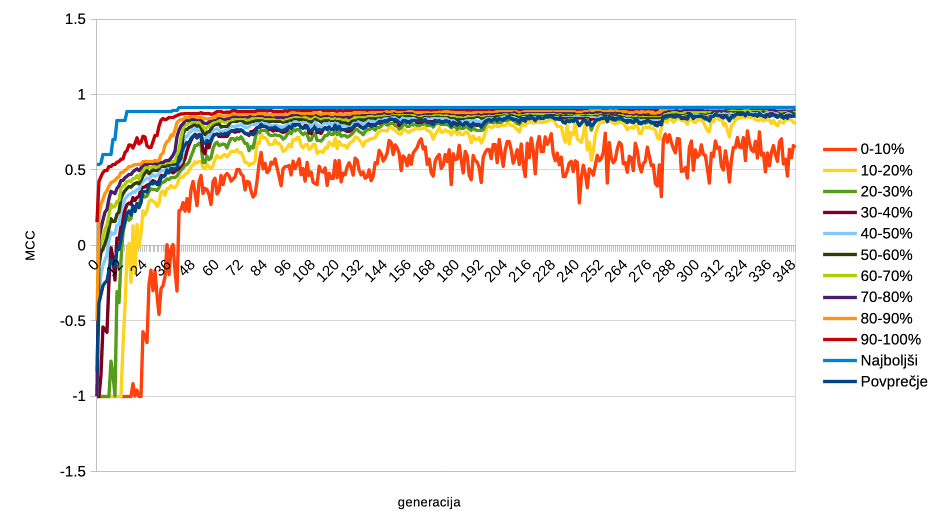
\includegraphics[width=13cm]{wine/2/mcc}
    \end{center}
    \caption{Graf MCC populacije najboljšega agenta drugega nabora skozi generacije.}
    \label{fig:wine_mcc_2}
\end{figure}

\begin{figure}[H]
    \begin{center}
        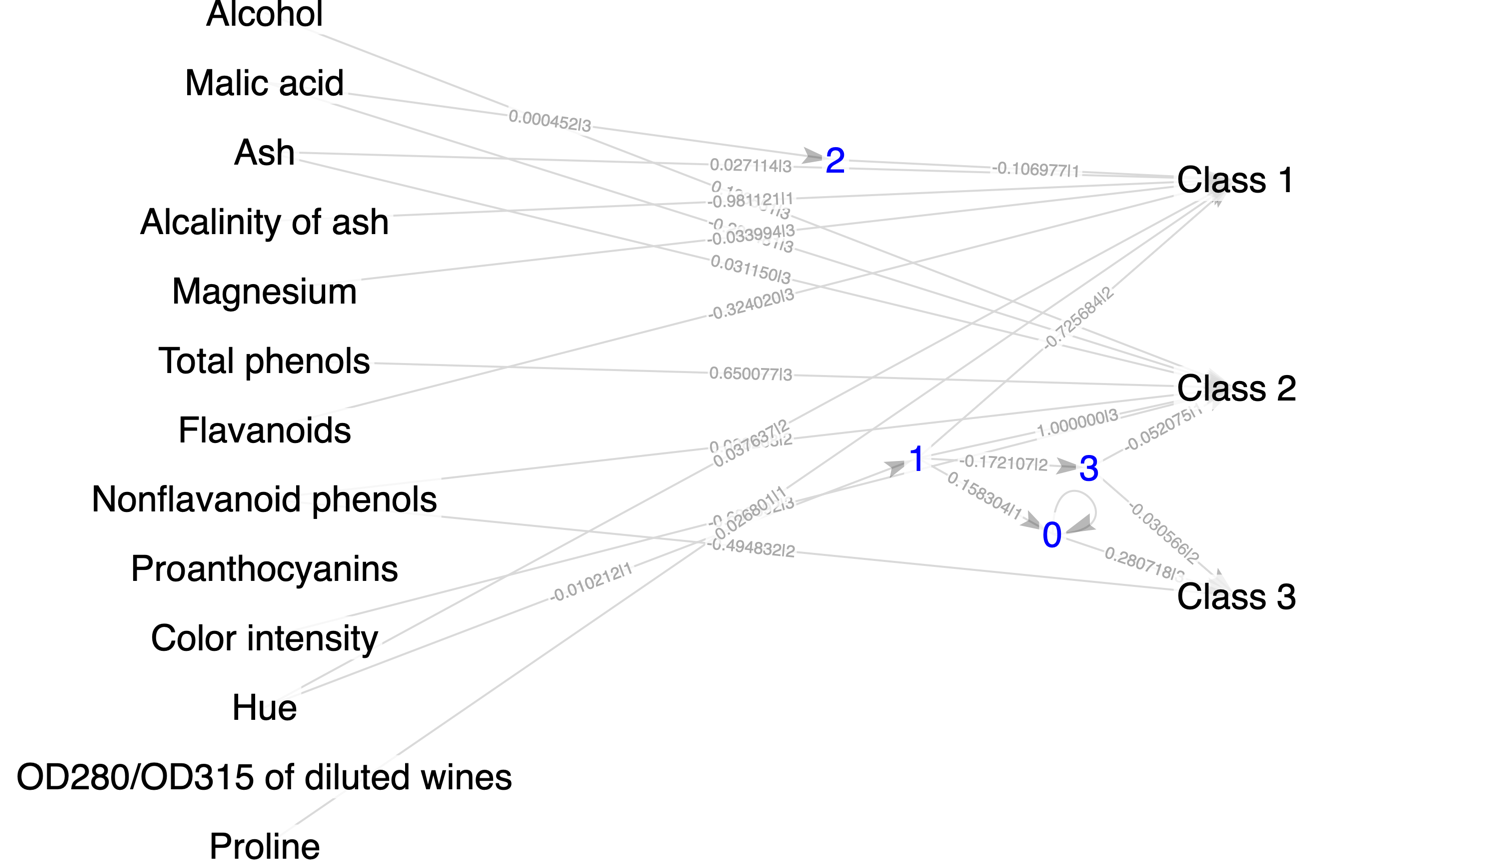
\includegraphics[width=13cm]{wine/2/acc_g}
    \end{center}
    \caption{Vizualizacija najbolj točnega agenta drugega nabora. Vsebuje 6 povezav.}
    \label{fig:wine_acc_2_g}
\end{figure}

\begin{figure}[H]
    \begin{center}
        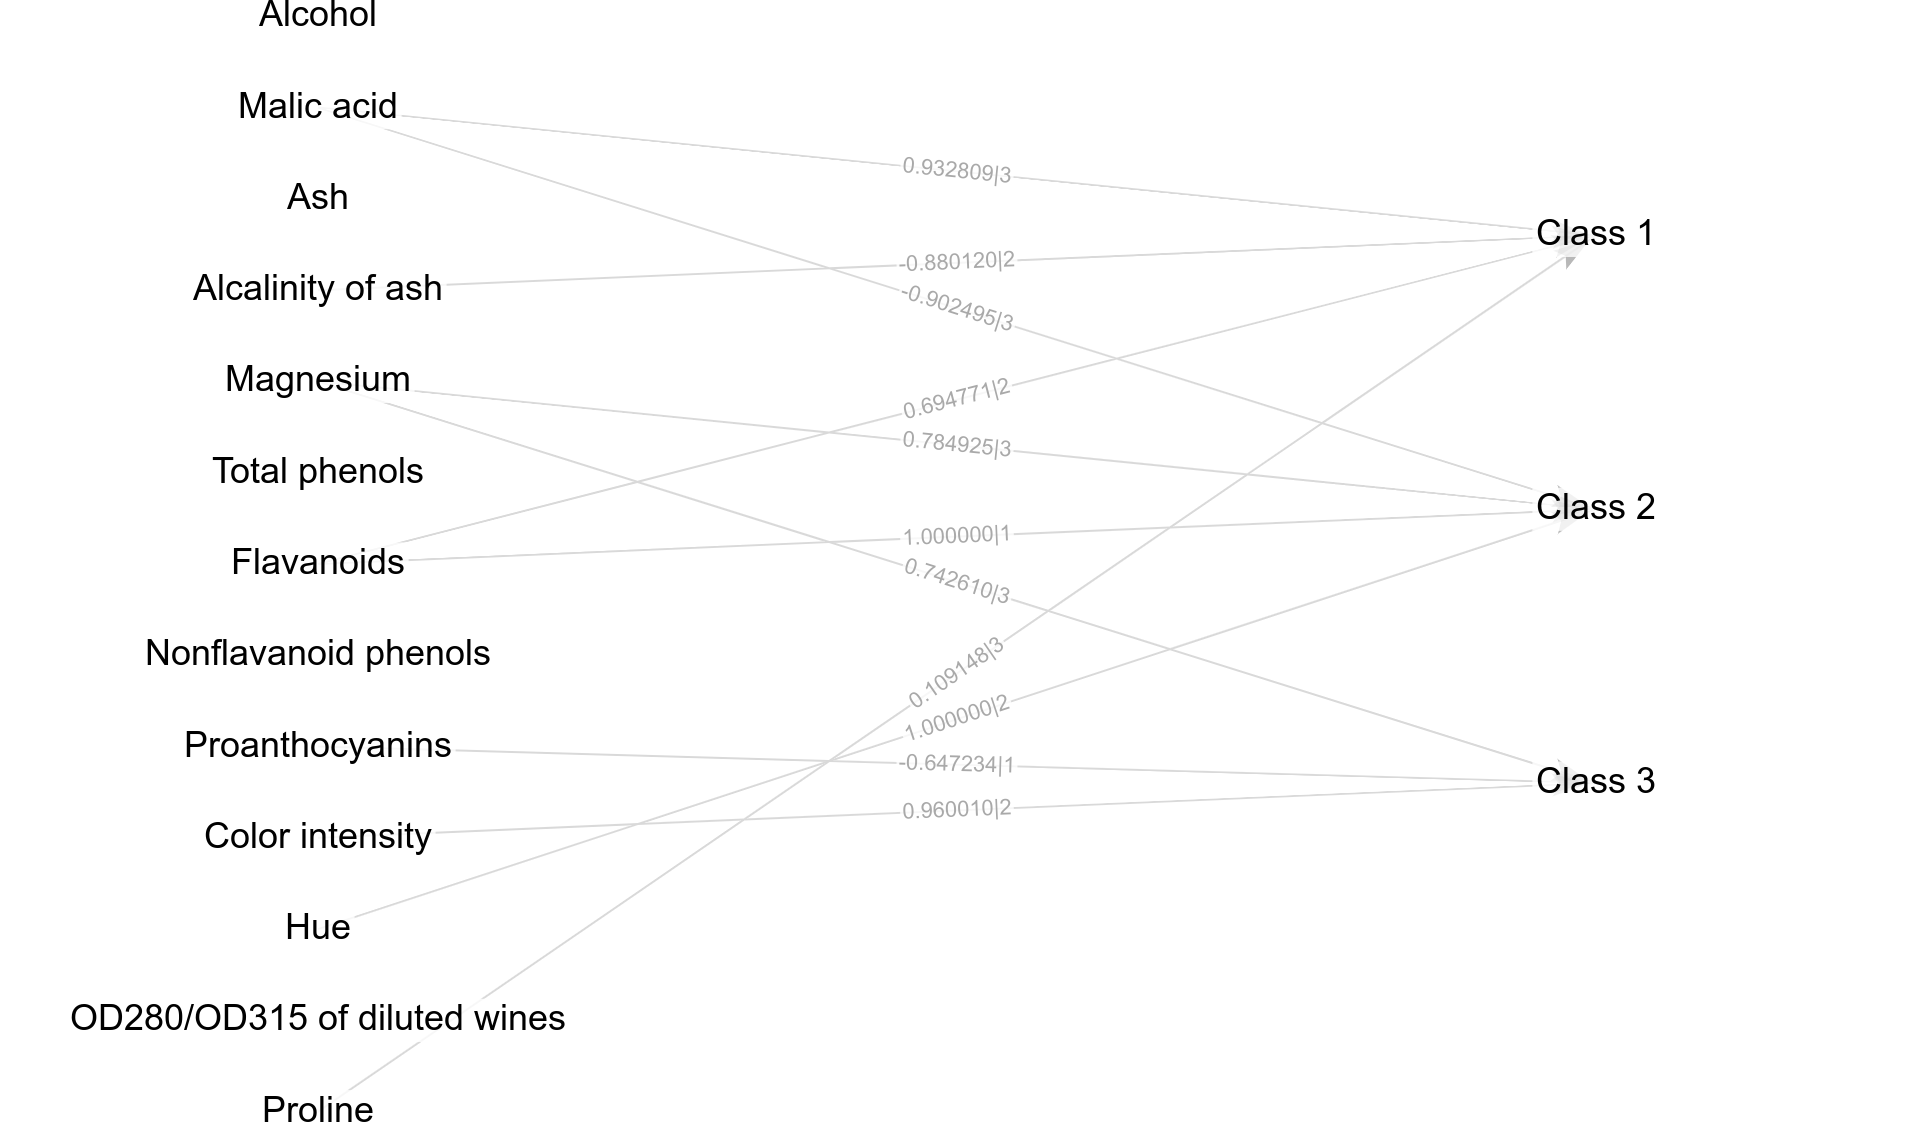
\includegraphics[width=13cm]{wine/2/mcc_g}
    \end{center}
    \caption{Vizualizacija agenta z največjim MCC drugega nabora. Vsebuje 1 globoko vozlišče in 7 povezav.}
    \label{fig:wine_mcc_2_g}
\end{figure}

\subsection{Tretji nabor}\label{subsec:dodatek-wine-tretji-nabor}
%%"/home/jure/CLionProjects/Neuroevolution/datasets/iris/iris.data" 350 25 75 4 true 0.1 175 true -0.001 -0.001 450 ACC
\begin{table}[H]
    \begin{center}
        \begin{tabular}{|| c | c c || c c ||}
            \hline
            \multirow{2}{*}{št. zagona} & \multicolumn{2}{c||}{točnost najboljšega agenta} & \multicolumn{2}{c||}{MCC najboljšega agenta} \\ \cline{2-5}
            & učna   & testna          & učna  & testna                  \\
            \hline
            1        & 80.0\% & 60.4\%          & 0.930 & 0.857                   \\
            \hline
            2        & 93.6\% & \textbf{96.2\%} & 0.906 & 0.860                   \\
            \hline
            3        & 95.2\% & 90.6\%          & 0.940 & 0.829                   \\
            \hline
            4        & 93.6\% & 88.7\%          & 0.774 & 0.763                   \\
            \hline
            5        & 88.0\% & 86.8\%          & 0.940 & \textbf{0.887 (92.5\%)} \\
            \hline
            $\sigma$ & 0.056  & 0.125           & 0.063 & 0.042                   \\
            \hline
        \end{tabular}
    \end{center}
    \caption{Rezultat tretjega nabora parametrov.}
    \label{tab:wine_result_3}
\end{table}

\begin{table}[H]
    \centering
    \begin{tabular}{||rcccc||}
        \hline
        razred  & Class 1 & Class 2 & Class 3 & vsota \\ \hline
        Class 1 & 18      & 0       & 0       & 18    \\ \hline
        Class 2 & 2       & 19      & 0       & 21    \\ \hline
        Class 3 & 0       & 0       & 14      & 14    \\ \hline
        vsota   & 20      & 19      & 14      & 53    \\ \hline
    \end{tabular}
    \caption{Matrika zmot najbolj točnega agenta tretjega nabora.}
    \label{tab:wine_acc_3}
\end{table}

\begin{table}[H]
    \centering
    \begin{tabular}{||rcccc||}
        \hline
        razred  & Class 1 & Class 2 & Class 3 & vsota \\ \hline
        Class 1 & 15      & 3       & 0       & 18    \\ \hline
        Class 2 & 1       & 20      & 0       & 21    \\ \hline
        Class 3 & 0       & 0       & 14      & 14    \\ \hline
        vsota   & 16      & 23      & 14      & 53    \\ \hline
    \end{tabular}
    \caption{Matrika zmot agenta z največjim MCC tretjega nabora.}
    \label{tab:wine_mcc_3}
\end{table}

\begin{figure}[H]
    \begin{center}
        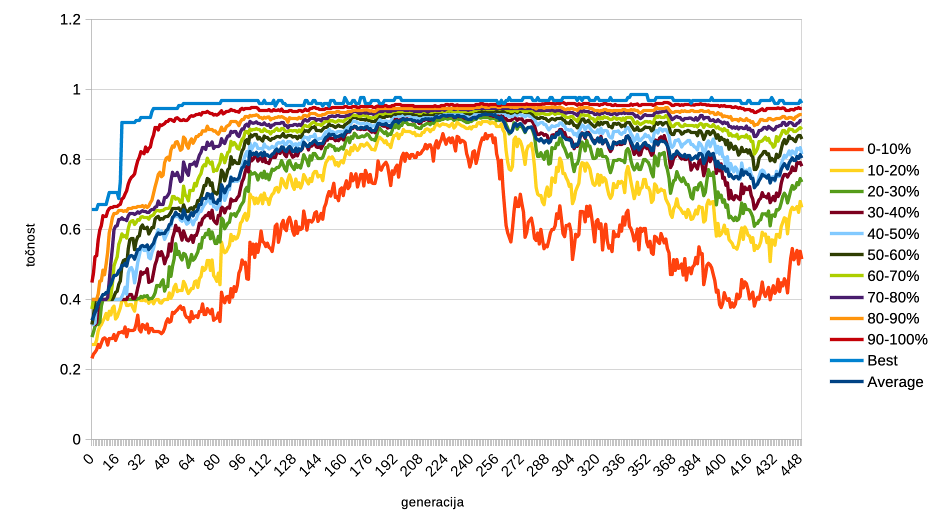
\includegraphics[width=13cm]{wine/3/acc}
    \end{center}
    \caption{Graf točnosti populacije najboljšega agenta tretjega nabora skozi generacije.}
    \label{fig:wine_acc_3}
\end{figure}

\begin{figure}[H]
    \begin{center}
        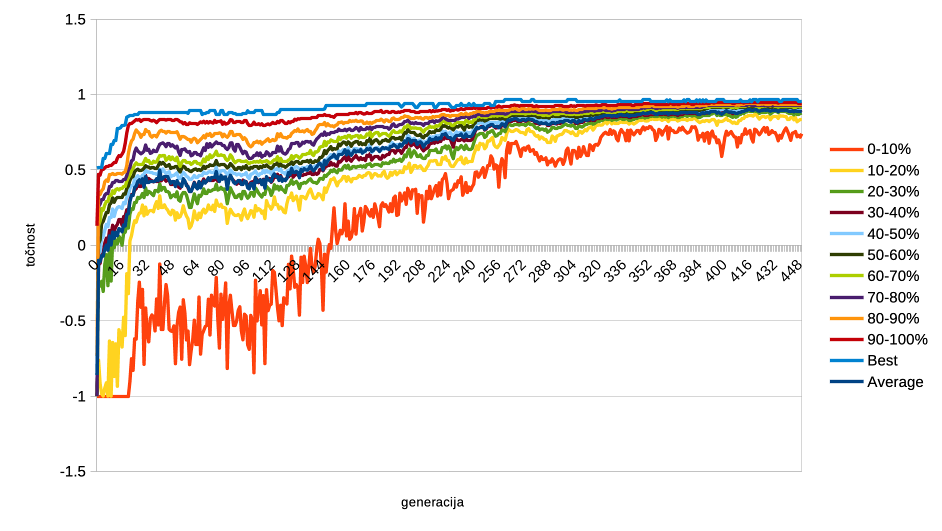
\includegraphics[width=13cm]{wine/3/mcc}
    \end{center}
    \caption{Graf MCC populacije najboljšega agenta tretjega nabora skozi generacije.}
    \label{fig:wine_mcc_3}
\end{figure}

\begin{figure}[H]
    \begin{center}
        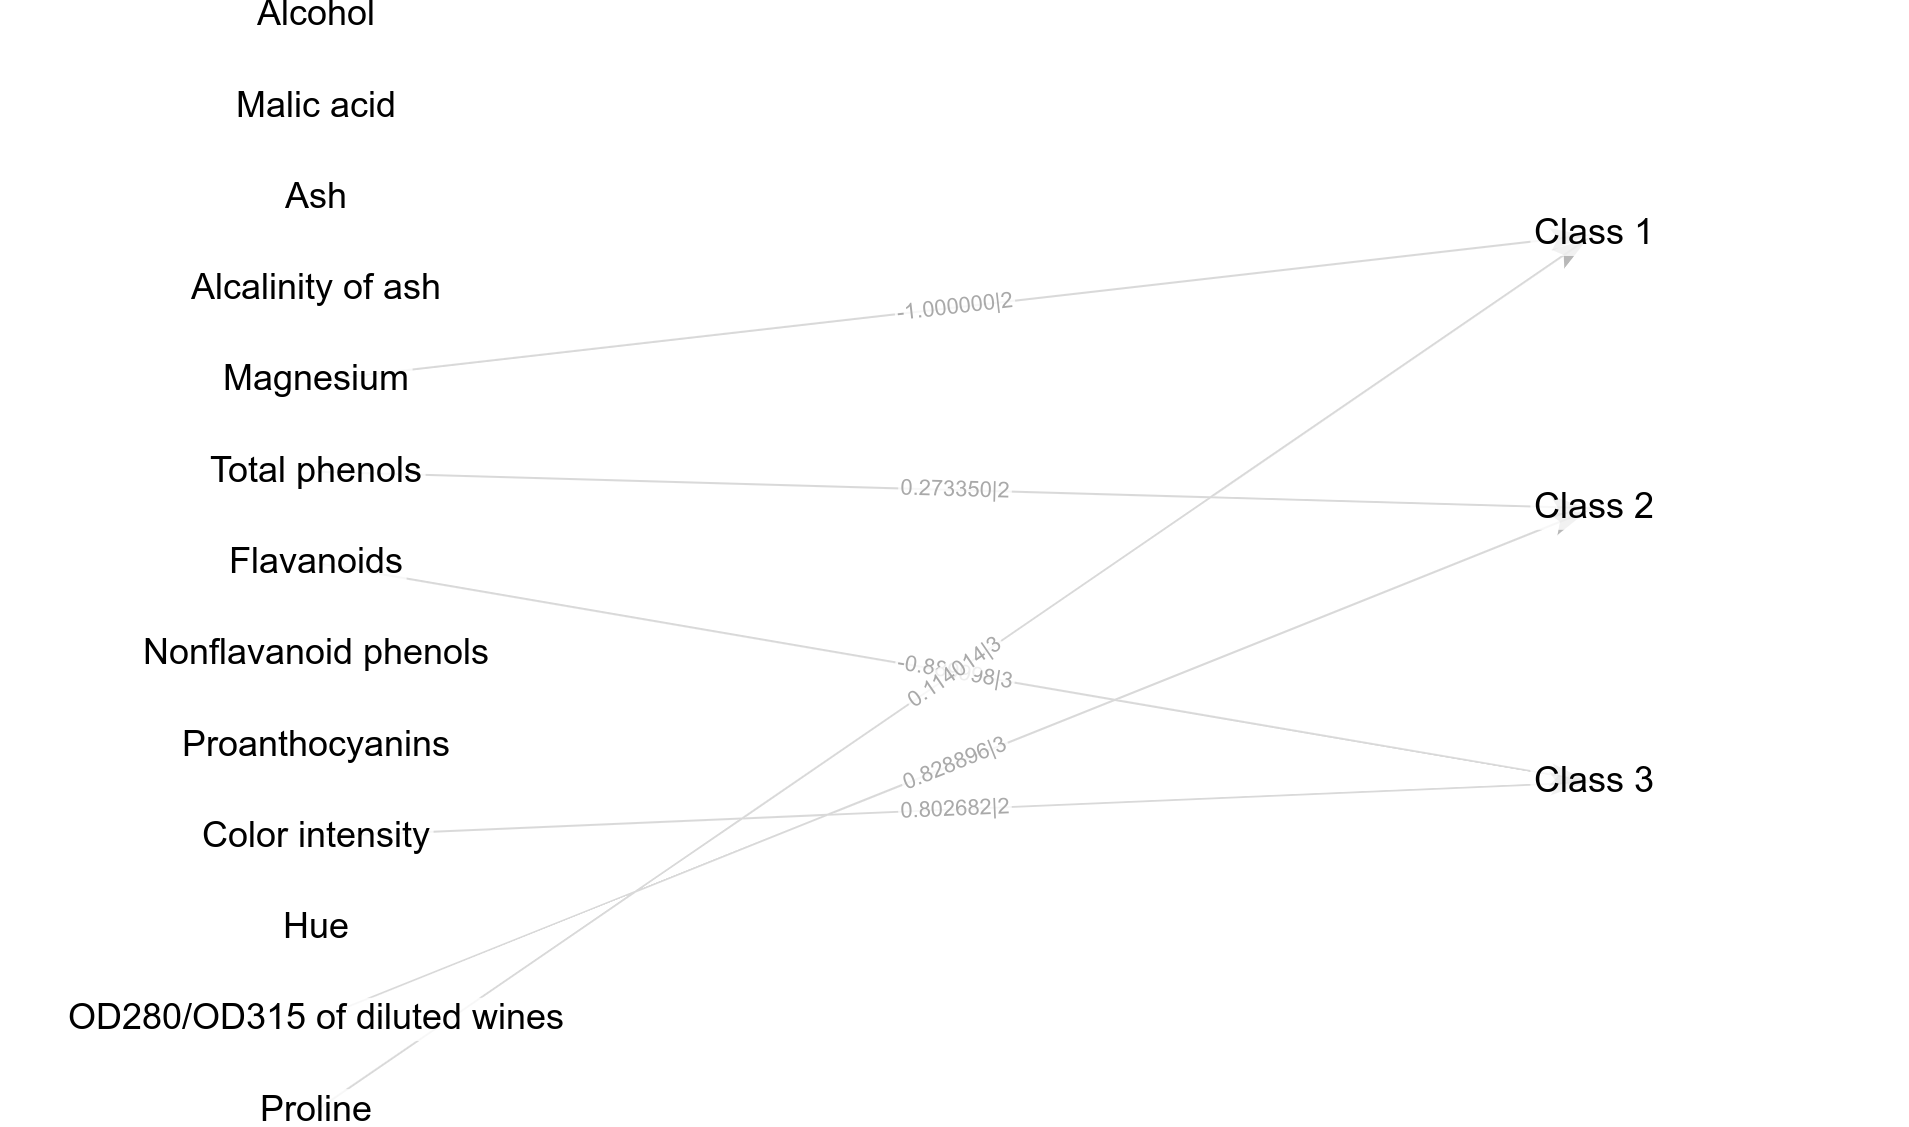
\includegraphics[width=13cm]{wine/3/acc_g}
    \end{center}
    \caption{Vizualizacija najbolj točnega agenta tretjega nabora. Vsebuje 11 povezav.}
    \label{fig:wine_acc_3_g}
\end{figure}

\begin{figure}[H]
    \begin{center}
        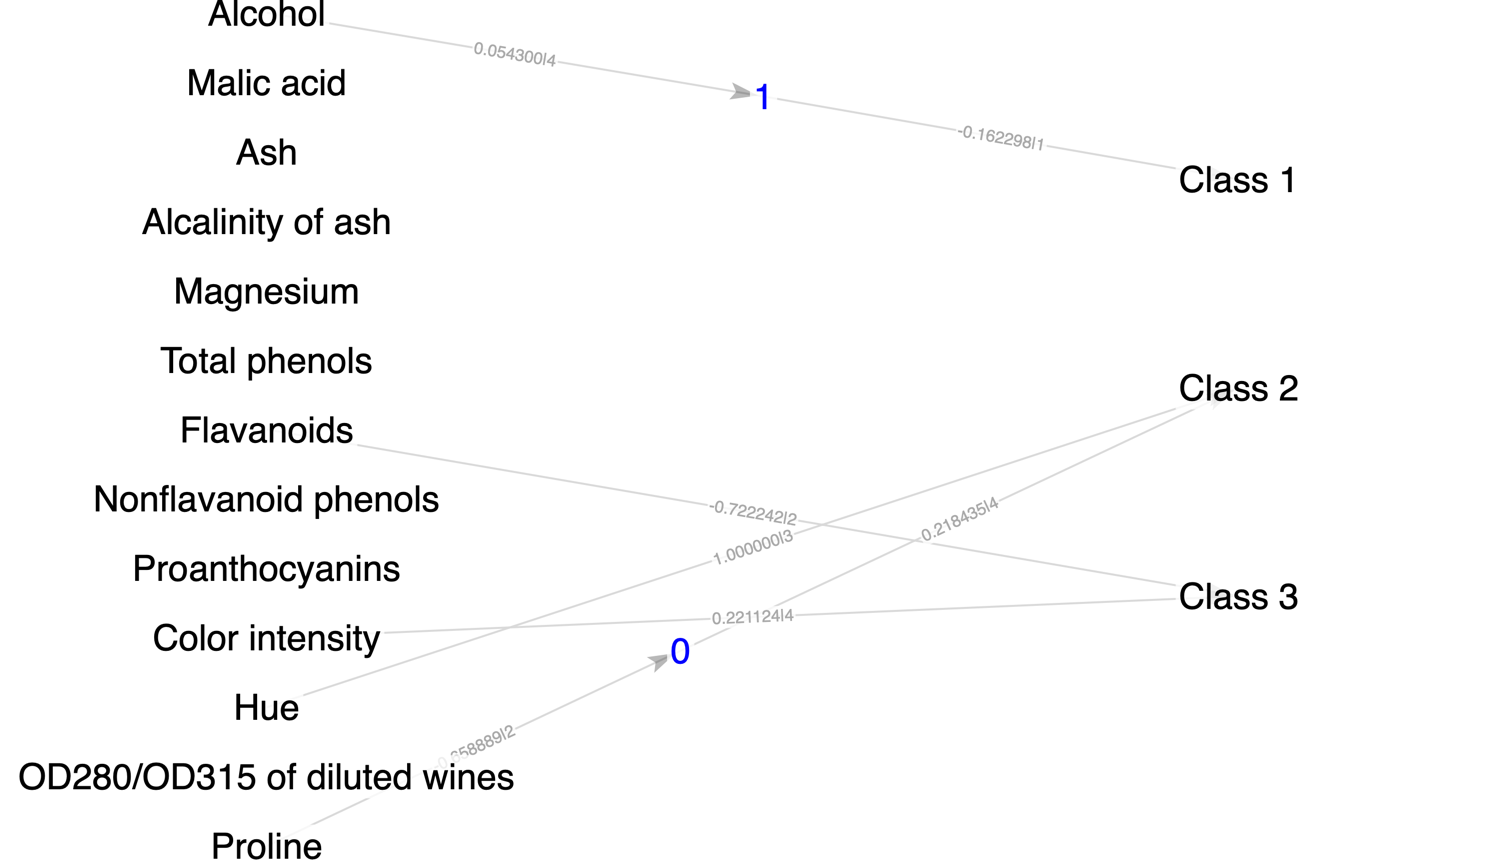
\includegraphics[width=13cm]{wine/3/mcc_g}
    \end{center}
    \caption{Vizualizacija agenta z največjim MCC tretjega nabora. Vsebuje 2 globoki vozlišči in 7 povezav.}
    \label{fig:wine_mcc_3_g}
\end{figure}

\section{Car Evaluation}\label{sec:dodatek-car-test}
%% arrowLength=10
%% linkWidth=3
%% input fy=50*node.pos
%% output fx=350
%% output fy=50*node.pos+50
%% MAX_FONT_SIZE=8
\begin{table}[H]
    \begin{center}
        \begin{tabular}{||l c c c||}
            \hline
            & 1        & 2        & 3 \\ [0.5ex]
            \hline
            velikost populacije              & 200      & 250      & 350      \\
            \hline
            največje število vmesnih vozlišč & 15       & 20       & 40       \\
            \hline
            največje število povezav         & 30       & 50       & 100      \\
            \hline
            največje število prečkanj        & 2        & 3        & 4        \\
            \hline
            delež mutiranih potomcev         & 10\%     & 10\%     & 10\%     \\
            \hline
            prispevek kompleksnosti          & -0.00001 & -0.00001 & -0.00001 \\
            \hline
            število generacij                & 200      & 200      & 300      \\
            \hline
        \end{tabular}
    \end{center}
    \caption{Nabori inicializacijskih parametrov poganjanja na množici Car Evaluation.}
    \label{tab:param_car}
\end{table}

\subsection{Prvi nabor}\label{subsec:dodatek-car-prvi-nabor}
%%"/home/jure/CLionProjects/Neuroevolution/datasets/car/car.data" 200 15 30 2 true 0.1 100 true -0.00001 200 ACC
\begin{table}[H]
    \begin{center}
        \begin{tabular}{|| c | c c || c c ||}
            \hline
            \multirow{2}{*}{št. zagona} & \multicolumn{2}{c||}{točnost najboljšega agenta} & \multicolumn{2}{c||}{MKK najboljšega agenta} \\ \cline{2-5}
            & učna   & testna          & učna  & testna                  \\
            \hline
            1         & 71.7\% & 71.4\%          & 0.507 & 0.454                   \\
            \hline
            2         & 72.6\% & 73.4\%          & 0.477 & 0.486                   \\
            \hline
            3         & 74.0\% & \textbf{73.6\%} & 0.457 & 0.431                   \\
            \hline
            4         & 71.4\% & 71.0\%          & 0.496 & \textbf{0.487 (73.7\%)} \\
            \hline
            5         & 72.1\% & 70.7\%          & 0.483 & 0.403                   \\
            \hline
            povprečje & 72.4\% & 72.0\%          & 0.478 & 0.452                   \\
            \hline
            $\sigma$  & 0.009  & 0.012           & 0.017 & 0.032                   \\
            \hline
        \end{tabular}
    \end{center}
    \caption{Rezultat prvega nabora parametrov.}
    \label{tab:car_result_1}
\end{table}

\begin{table}[H]
    \centering
    \begin{tabular}{||rccccc||}
        \hline
        razred       & unacceptable & acceptable & good & very good & vsota \\ \hline
        unacceptable & 354          & 0          & 9    & 0         & 363   \\ \hline
        acceptable   & 100          & 14         & 1    & 0         & 115   \\ \hline
        good         & 8            & 0          & 13   & 0         & 21    \\ \hline
        very good    & 10           & 1          & 8    & 0         & 19    \\ \hline
        vsota        & 472          & 15         & 31   & 0         & 518   \\ \hline
    \end{tabular}
    \caption{Matrika zmot najbolj točnega agenta prvega nabora. Agent ne more napovedati razreda \enquote{zelo dobro}.}
    \label{tab:car_acc_1}
\end{table}

\begin{table}[H]
    \centering
    \begin{tabular}{||rccccc||}
        \hline
        razred       & unacceptable & acceptable & good & very good & vsota \\ \hline
        unacceptable & 289          & 74         & 0    & 0         & 363   \\ \hline
        acceptable   & 22           & 93         & 0    & 0         & 115   \\ \hline
        good         & 0            & 21         & 0    & 0         & 21    \\ \hline
        very good    & 0            & 19         & 0    & 0         & 19    \\ \hline
        vsota        & 311          & 207        & 0    & 0         & 518   \\ \hline
    \end{tabular}
    \caption{Matrika zmot agenta z največjim MKK prvega nabora. Agent lahko napove samo razreda \enquote{nesprejemljivo} in \enquote{sprejemljivo}.}
    \label{tab:car_mcc_1}
\end{table}

\begin{figure}[H]
    \begin{center}
        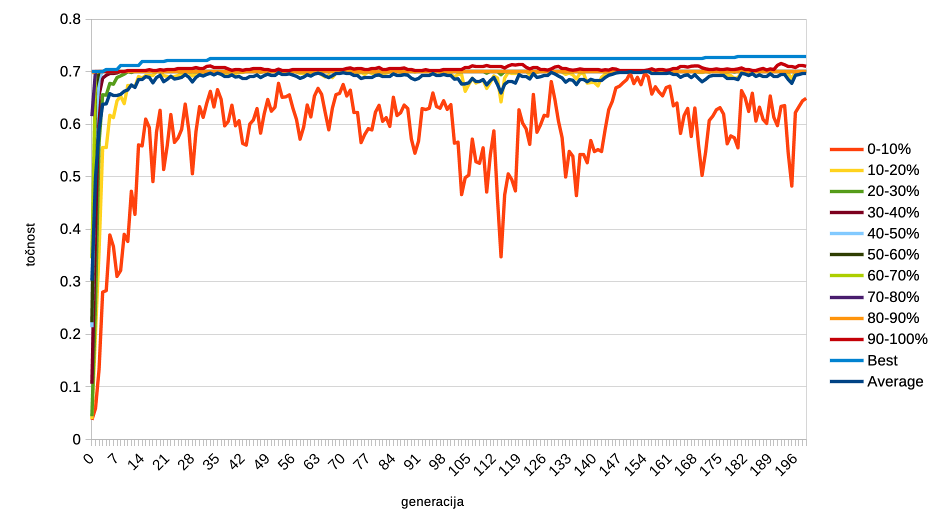
\includegraphics[width=13cm]{car/1/acc}
    \end{center}
    \caption{Graf točnosti populacije najboljšega agenta prvega nabora skozi generacije.}
    \label{fig:car_acc_1}
\end{figure}

\begin{figure}[H]
    \begin{center}
        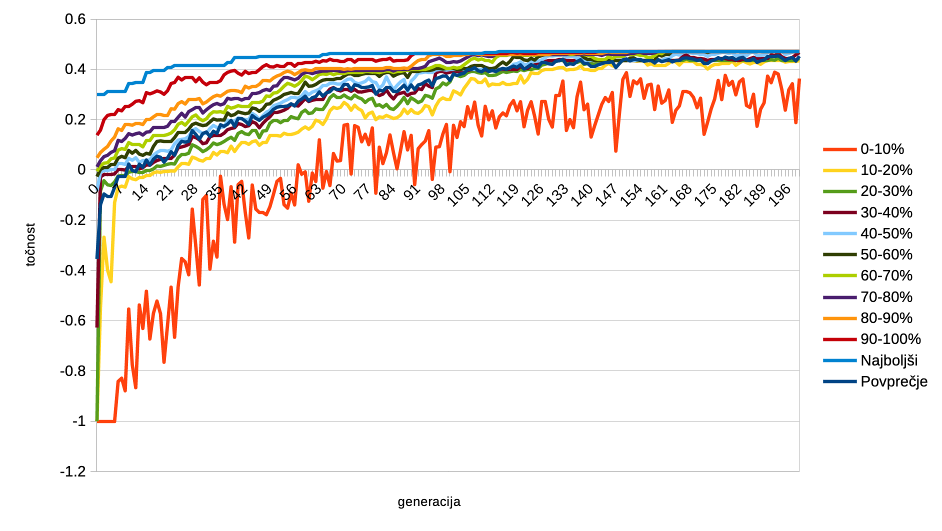
\includegraphics[width=13cm]{car/1/mcc}
    \end{center}
    \caption{Graf MKK populacije najboljšega agenta prvega nabora skozi generacije.}
    \label{fig:car_mcc_1}
\end{figure}

\begin{figure}[H]
    \begin{center}
        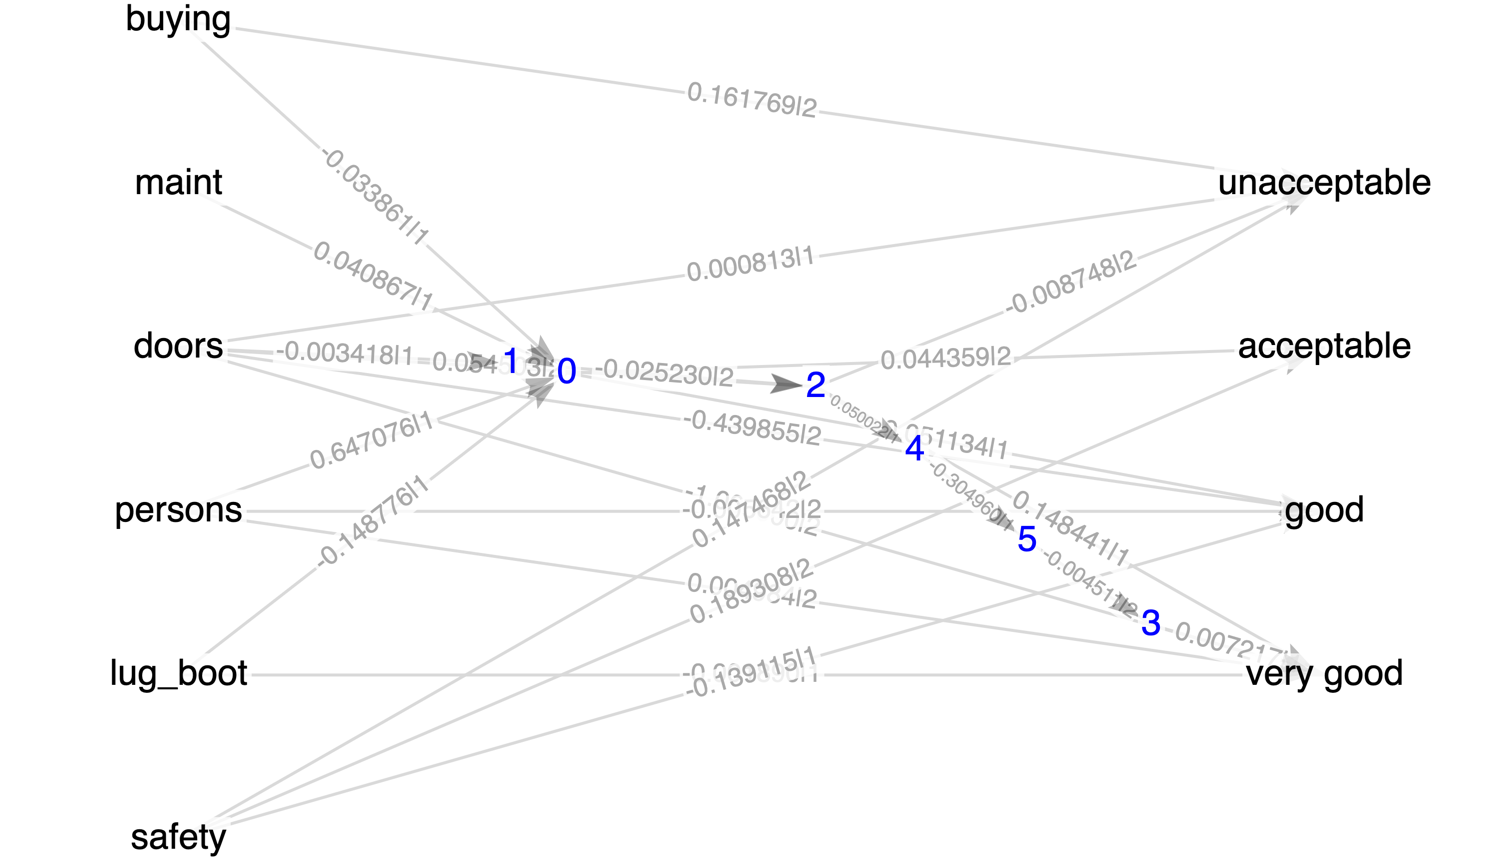
\includegraphics[width=13cm]{car/1/acc_g}
    \end{center}
    \caption{Vizualizacija najbolj točnega agenta prvega nabora. Vsebuje 10 povezav.}
    \label{fig:car_acc_1_g}
\end{figure}

\begin{figure}[H]
    \begin{center}
        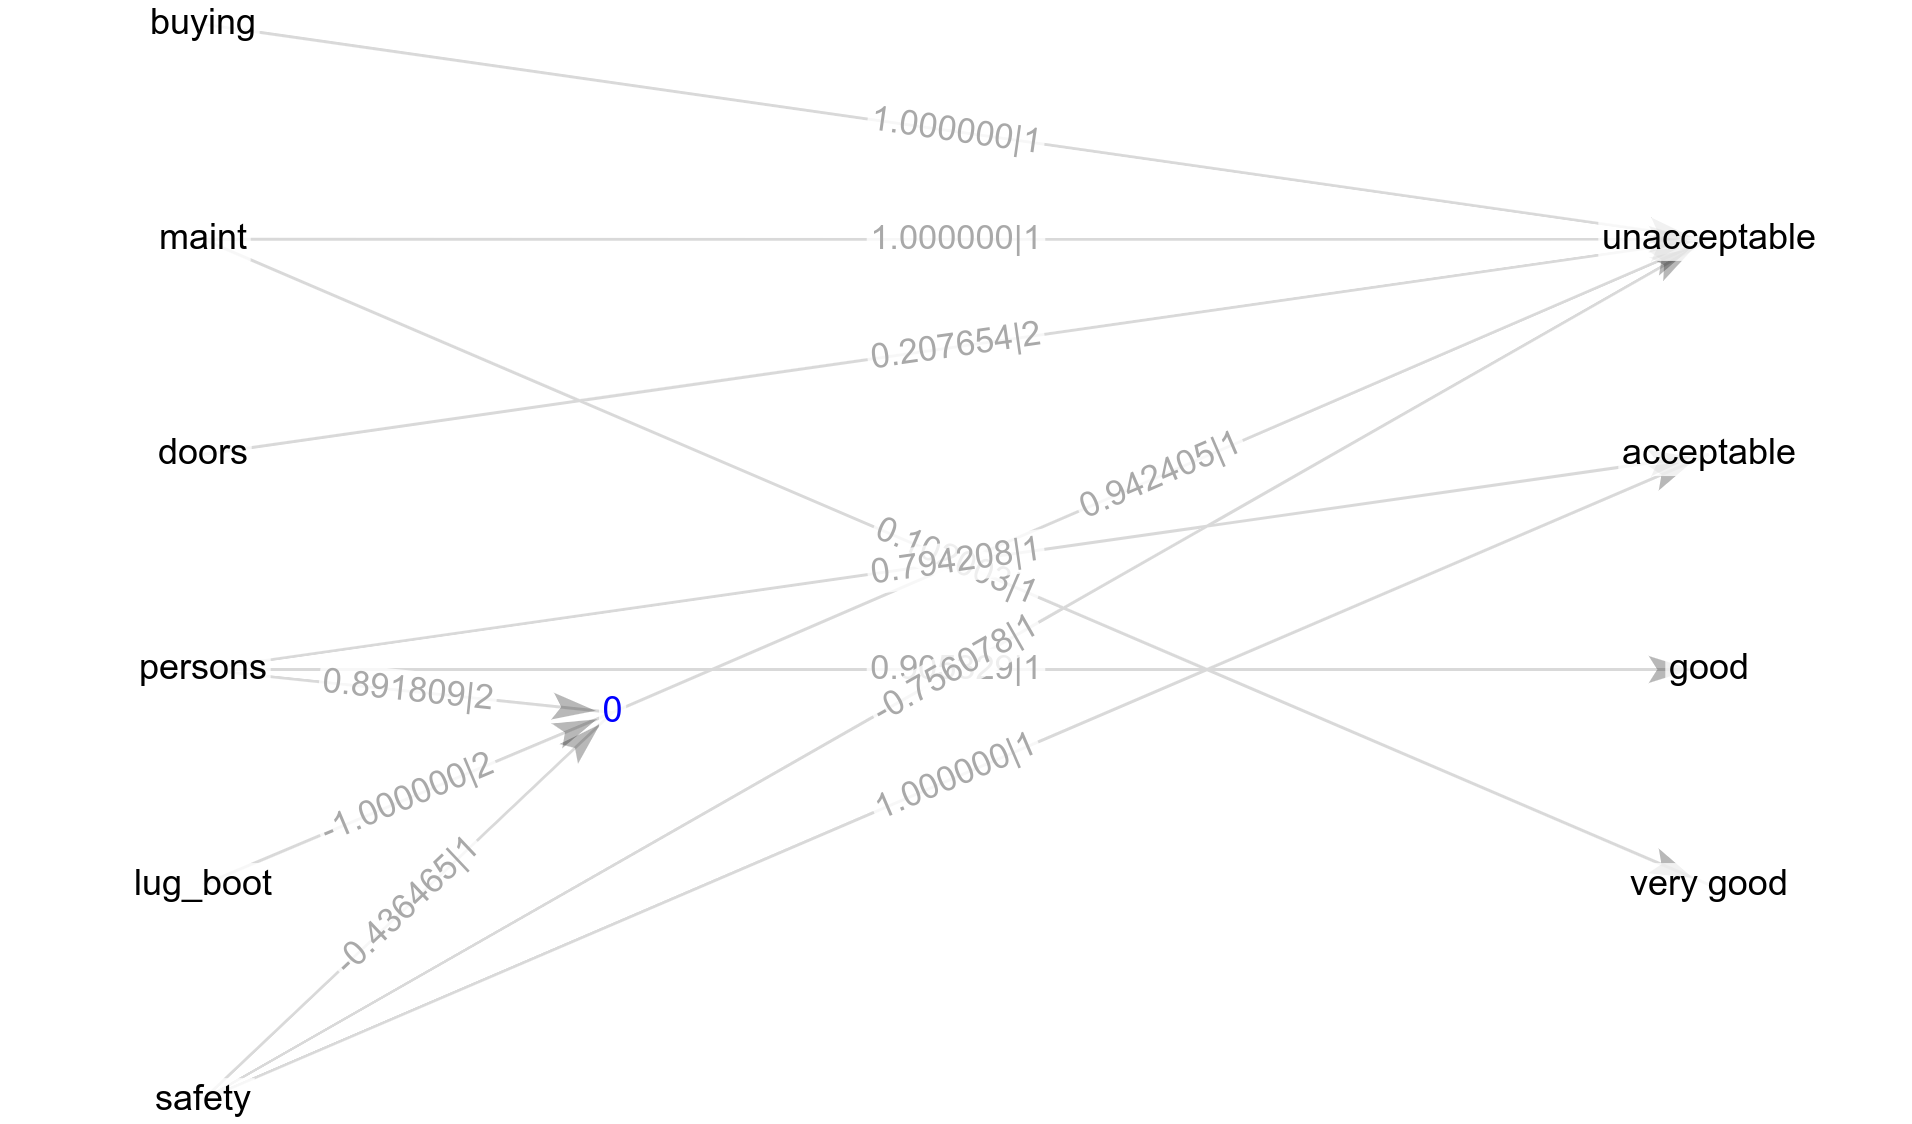
\includegraphics[width=13cm]{car/1/mcc_g}
    \end{center}
    \caption{Vizualizacija agenta z največjim MKK prvega nabora. Vsebuje 1 vmesno vozlišče in 12 povezav.}
    \label{fig:car_mcc_1_g}
\end{figure}

\subsection{Drugi nabor}\label{subsec:dodatek-car-drugi-nabor}
%% 250 20 50 3 true 0.1 125 true -0.00001 200 ACC
\begin{table}[H]
    \begin{center}
        \begin{tabular}{|| c | c c || c c ||}
            \hline
            \multirow{2}{*}{št. zagona} & \multicolumn{2}{c||}{točnost najboljšega agenta} & \multicolumn{2}{c||}{MKK najboljšega agenta} \\ \cline{2-5}
            & učna   & testna          & učna  & testna                  \\
            \hline
            1         & 76.6\% & \textbf{74.3\%} & 0.502 & 0.470                   \\
            \hline
            2         & 74.9\% & 68.3\%          & 0.481 & 0.484                   \\
            \hline
            3         & 71.9\% & 72.0\%          & 0.485 & 0.493                   \\
            \hline
            4         & 72.3\% & 72.8\%          & 0.565 & \textbf{0.585 (75.9\%)} \\
            \hline
            5         & 72.3\% & 71.0\%          & 0.492 & 0.457                   \\
            \hline
            povprečje & 73.6\% & 71.7\%          & 0.505 & 0.498                   \\
            \hline
            $\sigma$  & 0.018  & 0.020            & 0.031 & 0.045                   \\
            \hline
        \end{tabular}
    \end{center}
    \caption{Rezultat drugega nabora parametrov.}
    \label{tab:car_result_2}
\end{table}

\begin{table}[H]
    \centering
    \begin{tabular}{||rccccc||}
        \hline
        razred       & unacceptable & acceptable & good & very good & vsota \\ \hline
        unacceptable & 325          & 38         & 0    & 0         & 363   \\ \hline
        acceptable   & 55           & 60         & 0    & 0         & 115   \\ \hline
        good         & 0            & 21         & 0    & 0         & 21    \\ \hline
        very good    & 0            & 19         & 0    & 0         & 19    \\ \hline
        vsota        & 380          & 138        & 0    & 0         & 518   \\ \hline
    \end{tabular}
    \caption{Matrika zmot najbolj točnega agenta drugega nabora. Agent lahko napove samo razreda \enquote{nesprejemljivo} in \enquote{sprejemljivo}.}
    \label{tab:car_acc_2}
\end{table}

\begin{table}[H]
    \centering
    \begin{tabular}{||rccccc||}
        \hline
        razred       & unacceptable & acceptable & good & very good & vsota \\ \hline
        unacceptable & 271          & 67         & 0    & 25        & 363   \\ \hline
        acceptable   & 7            & 107        & 0    & 1         & 115   \\ \hline
        good         & 0            & 9          & 0    & 12        & 21    \\ \hline
        very good    & 0            & 4          & 0    & 15        & 19    \\ \hline
        vsota        & 278          & 187        & 0    & 53        & 518   \\ \hline
    \end{tabular}
    \caption{Matrika zmot agenta z največjim MKK drugega nabora. Agent ne more napovedati razreda \enquote{dobro}.}
    \label{tab:car_mcc_2}
\end{table}

\begin{figure}[H]
    \begin{center}
        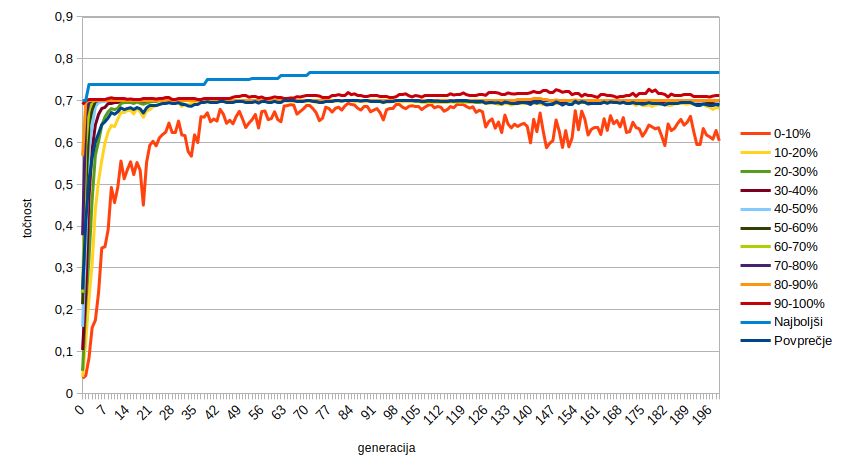
\includegraphics[width=13cm]{car/2/acc}
    \end{center}
    \caption{Graf točnosti populacije najboljšega agenta drugega nabora skozi generacije.}
    \label{fig:car_acc_2}
\end{figure}

\begin{figure}[H]
    \begin{center}
        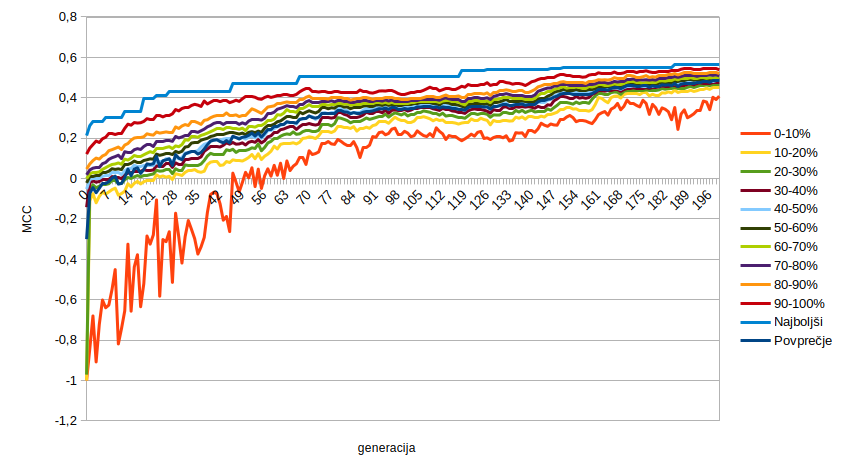
\includegraphics[width=13cm]{car/2/mcc}
    \end{center}
    \caption{Graf MKK populacije najboljšega agenta drugega nabora skozi generacije.}
    \label{fig:car_mcc_2}
\end{figure}

\begin{figure}[H]
    \begin{center}
        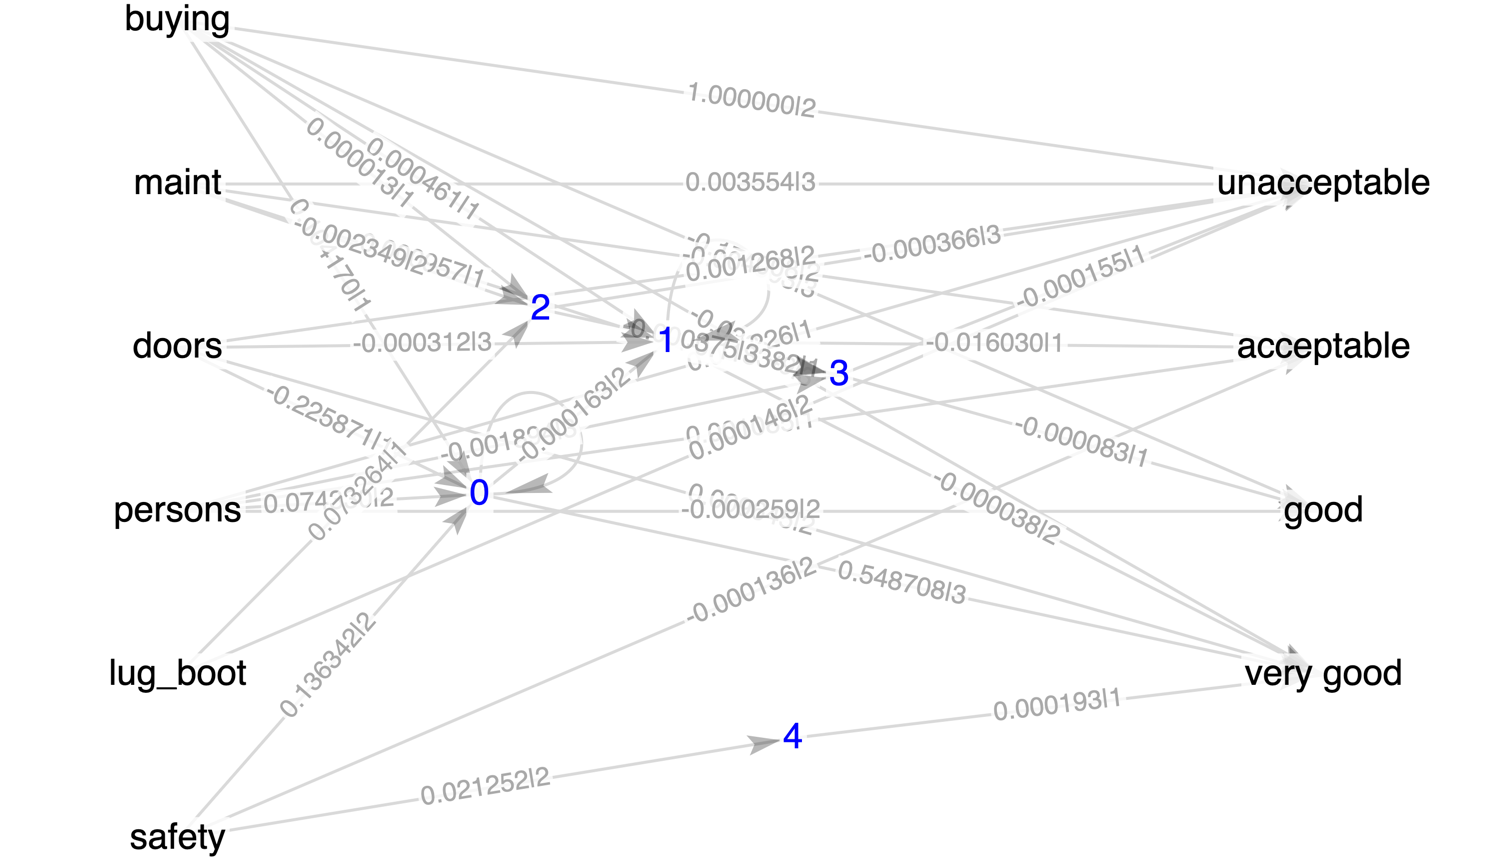
\includegraphics[width=13cm]{car/2/acc_g}
    \end{center}
    \caption{Vizualizacija najbolj točnega agenta drugega nabora. Vsebuje 1 vmesno vozlišče in 16 povezav.}
    \label{fig:car_acc_2_g}
\end{figure}

\begin{figure}[H]
    \begin{center}
        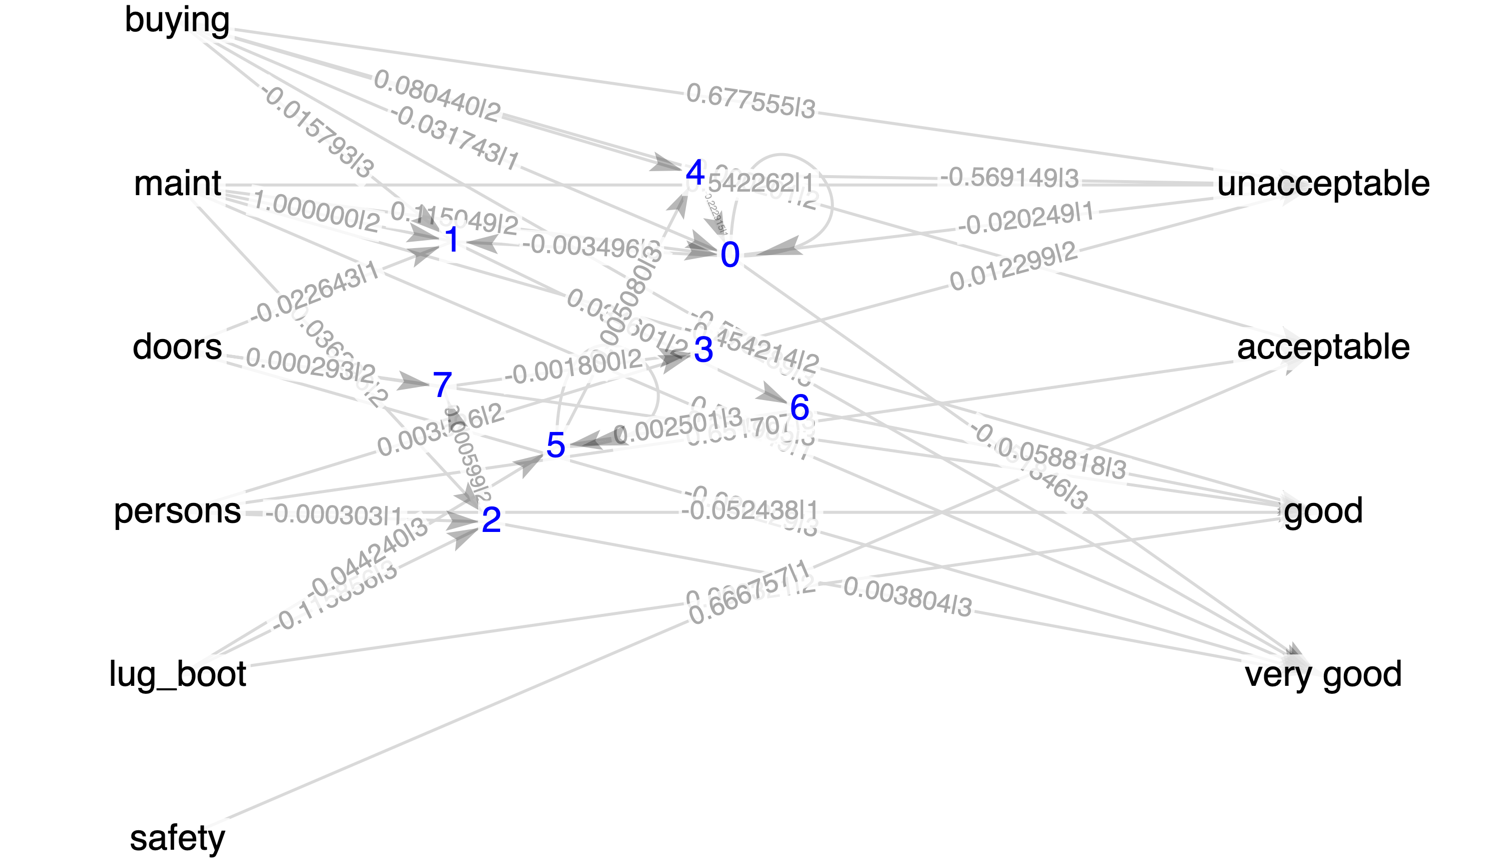
\includegraphics[width=13cm]{car/2/mcc_g}
    \end{center}
    \caption{Vizualizacija agenta z največjim MKK drugega nabora. Vsebuje 13 povezav.}
    \label{fig:car_mcc_2_g}
\end{figure}

\newpage

\subsection{Tretji nabor}\label{subsec:dodatek-car-tretji-nabor}
%% 350 40 100 4 true 0.1 175 true -0.00001 300 ACC
\begin{table}[H]
    \begin{center}
        \begin{tabular}{|| c | c c || c c ||}
            \hline
            \multirow{2}{*}{št. zagona} & \multicolumn{2}{c||}{točnost najboljšega agenta} & \multicolumn{2}{c||}{MKK najboljšega agenta} \\ \cline{2-5}
            & učna   & testna          & učna  & testna                  \\
            \hline
            1         & 73.6\% & \textbf{73.6\%} & 0.510 & 0.498                   \\
            \hline
            2         & 73.1\% & 71.2\%          & 0.486 & 0.502                   \\
            \hline
            3         & 72.4\% & 70.8\%          & 0.493 & 0.462                   \\
            \hline
            4         & 73.5\% & 72.0\%          & 0.468 & 0.467                   \\
            \hline
            5         & 72.7\% & 72.8\%          & 0.516 & \textbf{0.539 (73.7\%)} \\
            \hline
            povprečje & 73.1\% & 72.1\%          & 0.495 & 0.494                   \\
            \hline
            $\sigma$  & 0.005  & 0.010           & 0.017 & 0.028                   \\
            \hline
        \end{tabular}
    \end{center}
    \caption{Rezultat tretjega nabora parametrov.}
    \label{tab:car_result_3}
\end{table}

\begin{table}[H]
    \centering
    \begin{tabular}{||rccccc||}
        \hline
        razred       & unacceptable & acceptable & good & very good & vsota \\ \hline
        unacceptable & 325          & 38         & 0    & 0         & 363   \\ \hline
        acceptable   & 59           & 56         & 0    & 0         & 115   \\ \hline
        good         & 4            & 17         & 0    & 0         & 21    \\ \hline
        very good    & 0            & 19         & 0    & 0         & 19    \\ \hline
        vsota        & 388          & 130        & 0    & 0         & 518   \\ \hline
    \end{tabular}
    \caption{Matrika zmot najbolj točnega agenta tretjega nabora. Agent lahko napove samo razreda \enquote{nesprejemljivo} in \enquote{sprejemljivo}.}
    \label{tab:car_acc_3}
\end{table}

\begin{table}[H]
    \centering
    \begin{tabular}{||rccccc||}
        \hline
        razred       & unacceptable & acceptable & good & very good & vsota \\ \hline
        unacceptable & 270          & 66         & 0    & 27        & 363   \\ \hline
        acceptable   & 10           & 103        & 0    & 2         & 115   \\ \hline
        good         & 0            & 10         & 0    & 11        & 21    \\ \hline
        very good    & 0            & 10         & 0    & 9         & 19    \\ \hline
        vsota        & 280          & 189        & 0    & 49        & 518   \\ \hline
    \end{tabular}
    \caption{Matrika zmot agenta z največjim MKK tretjega nabora. Agent ne more napovedati razreda \enquote{dobro}.}
    \label{tab:car_mcc_3}
\end{table}

\begin{figure}[H]
    \begin{center}
        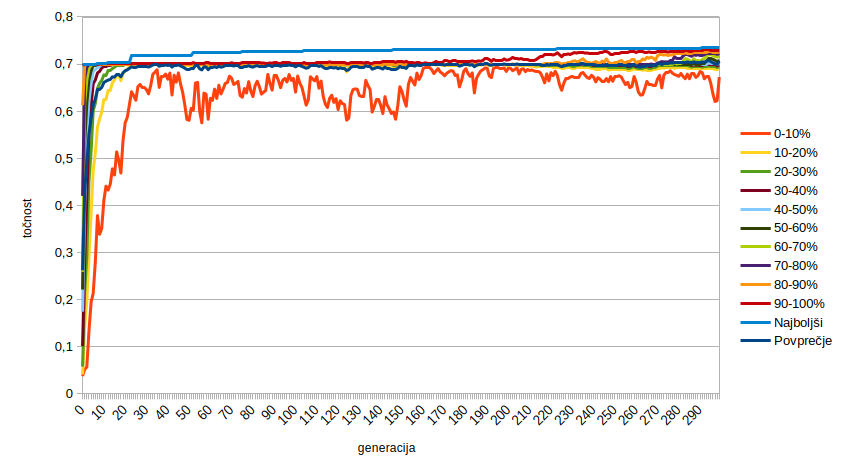
\includegraphics[width=13cm]{car/3/acc}
    \end{center}
    \caption{Graf točnosti populacije najboljšega agenta tretjega nabora skozi generacije.}
    \label{fig:car_acc_3}
\end{figure}

\begin{figure}[H]
    \begin{center}
        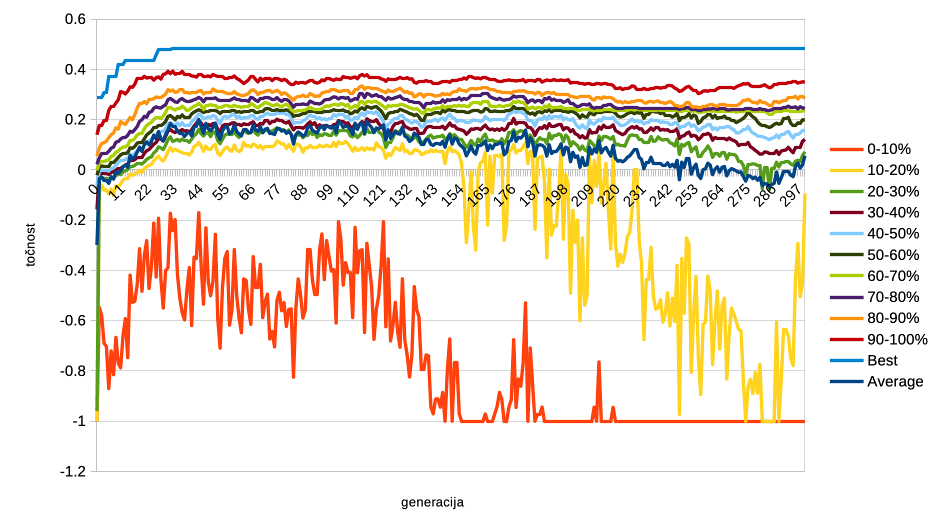
\includegraphics[width=13cm]{car/3/mcc}
    \end{center}
    \caption{Graf MKK populacije najboljšega agenta tretjega nabora skozi generacije.}
    \label{fig:car_mcc_3}
\end{figure}

\begin{figure}[H]
    \begin{center}
        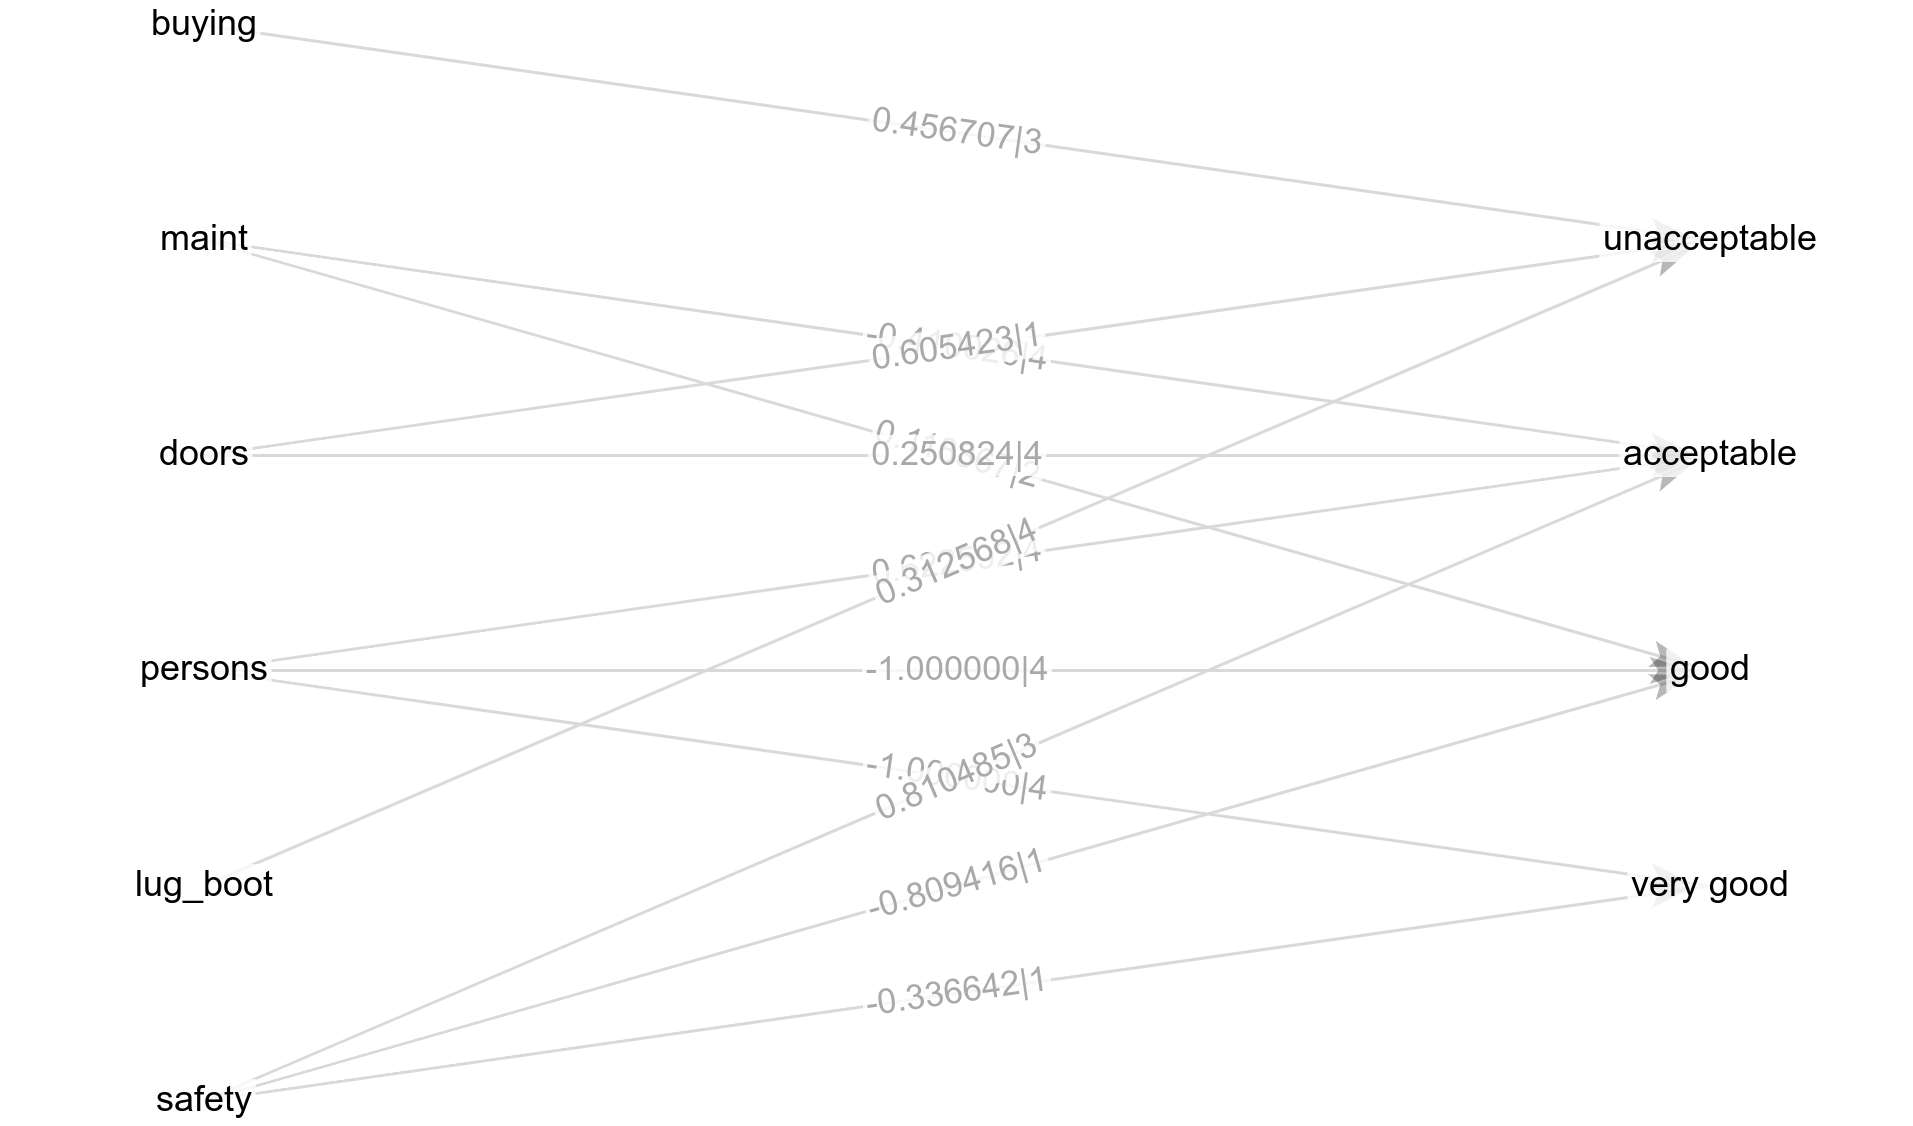
\includegraphics[width=13cm]{car/3/acc_g}
    \end{center}
    \caption{Vizualizacija najbolj točnega agenta tretjega nabora. Vsebuje 12 povezav.}
    \label{fig:car_acc_3_g}
\end{figure}

\begin{figure}[H]
    \begin{center}
        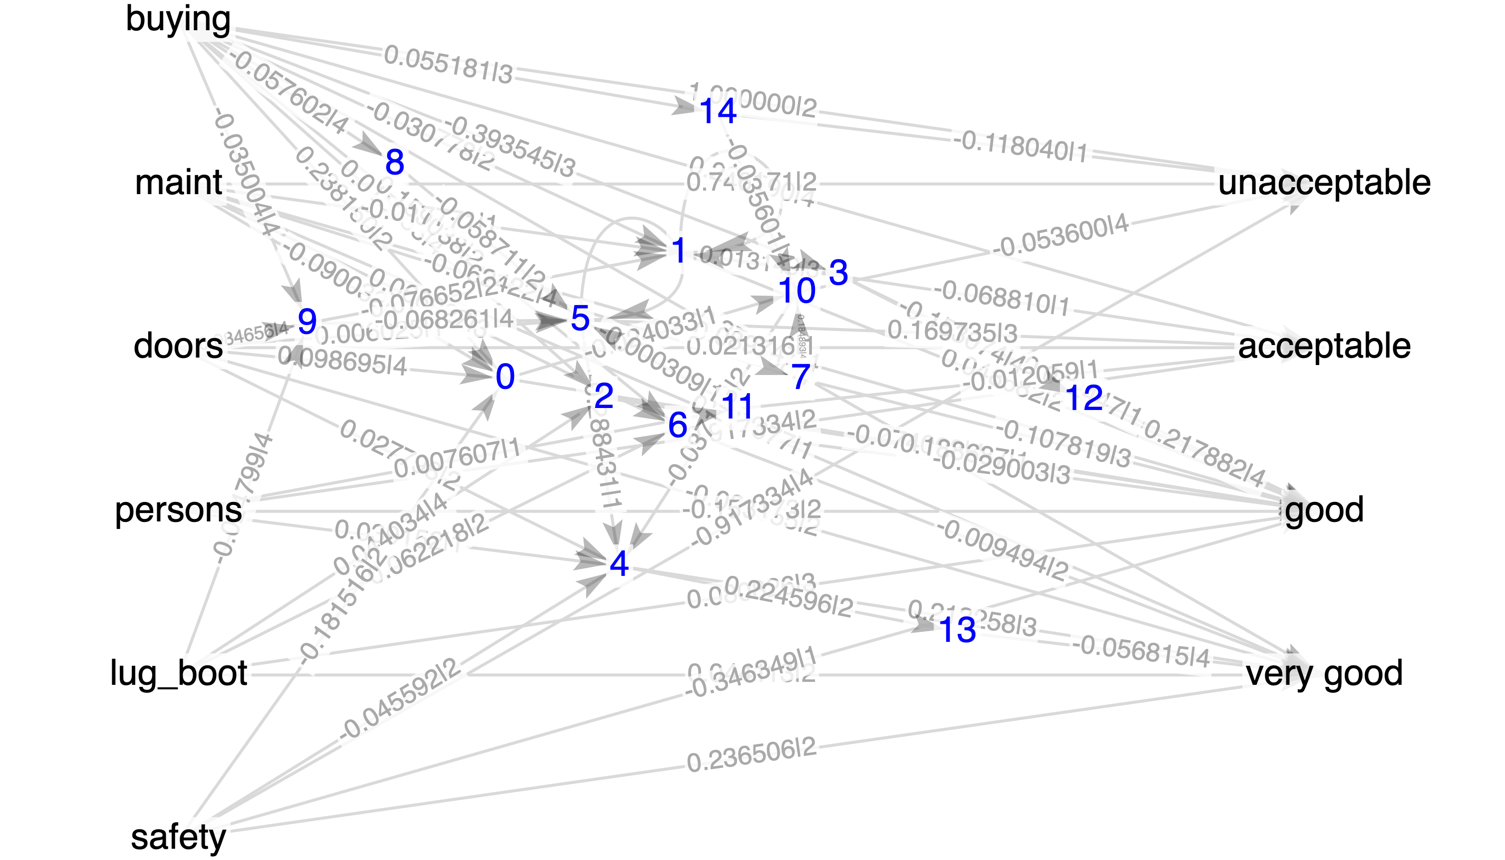
\includegraphics[width=13cm]{car/3/mcc_g}
    \end{center}
    \caption{Vizualizacija agenta z največjim MKK drugega nabora. Vsebuje 13 povezav.}
    \label{fig:car_mcc_3_g}
\end{figure}

\section{Shuttle}\label{sec:dodatek-statlog-test}
%% arrowLength=10
%% linkWidth=3
%% input fy=50*node.pos
%% output fx=550
%% output fy=50*node.pos+25
%% MAX_FONT_SIZE=8
Imena razredov v glavah matrik zmot so okrajšana zaradi formatiranja dokumenta.
\begin{table}[H]
    \begin{center}
        \begin{tabular}{||l c c c||}
            \hline
            & 1        & 2        & 3 \\ [0.5ex]
            \hline
            velikost populacije               & 200      & 250      & 350      \\
            \hline
            največje število globokih vozlišč & 15       & 20       & 40       \\
            \hline
            največje število povezav          & 30       & 50       & 100      \\
            \hline
            največje število prečkanj         & 2        & 3        & 4        \\
            \hline
            delež mutiranih potomcev          & 10\%     & 10\%     & 10\%     \\
            \hline
            prispevek kompleksnosti           & -0.00001 & -0.00001 & -0.00001 \\
            \hline
            število generacij                 & 200      & 250      & 300      \\
            \hline
        \end{tabular}
    \end{center}
    \caption{Nabori inicializacijskih parametrov poganjanja na množici Shuttle.}
    \label{tab:param_statlog}
\end{table}

\subsection{Prvi nabor}\label{subsec:dodatek-statlog-prvi-nabor}
%% branch shuttle
%% 200 15 30 2 true 0.1 100 true -0.00001 200 ACC
\begin{table}[H]
    \begin{center}
        \begin{tabular}{|| c | c c || c c ||}
            \hline
            \multirow{2}{*}{št. zagona} & \multicolumn{2}{c||}{točnost najboljšega agenta} & \multicolumn{2}{c||}{MCC najboljšega agenta} \\ \cline{2-5}
            & učna   & testna          & učna  & testna                  \\
            \hline
            1        & 91.3\% & 91.8\%          & 0.656 & 0.658                   \\
            \hline
            2        & 86.2\% & 86.8\%          & 0.628 & 0.632                   \\
            \hline
            3        & 84.0\% & 84.7\%          & 0.753 & \textbf{0.760 (92.1\%)} \\
            \hline
            4        & 86.8\% & 87.4\%          & 0.572 & 0.578                   \\
            \hline
            5        & 91.8\% & \textbf{92.4\%} & 0.744 & 0.752                   \\
            \hline
            $\sigma$ & 0.030  & 0.030           & 0.069 & 0.070                   \\
            \hline
        \end{tabular}
    \end{center}
    \caption{Rezultat prvega nabora parametrov.}
    \label{tab:statlog_result_1}
\end{table}

\begin{table}[H]
    \centering
    \begin{tabular}{||rcccccccc||}
        \hline
        razred    & RF    & FC & FO & High & Bypass & BC & BO & vsota \\ \hline
        Rad Flow  & 11405 & 0  & 10 & 61   & 1      & 1  & 0  & 11478 \\ \hline
        Fpv Close & 8     & 0  & 0  & 5    & 0      & 0  & 0  & 13    \\ \hline
        Fpv Open  & 11    & 0  & 21 & 6    & 1      & 0  & 0  & 39    \\ \hline
        High      & 998   & 0  & 0  & 1157 & 0      & 0  & 0  & 2155  \\ \hline
        Bypass    & 0     & 0  & 0  & 0    & 808    & 1  & 0  & 809   \\ \hline
        Bpv Close & 1     & 0  & 0  & 1    & 2      & 0  & 0  & 4     \\ \hline
        Bpv Open  & 0     & 0  & 2  & 0    & 0      & 0  & 0  & 2     \\ \hline
        vsota     & 12423 & 0  & 33 & 1230 & 812    & 2  & 0  & 14500 \\ \hline
    \end{tabular}
    \caption{Matrika zmot najbolj točnega agenta prvega nabora. Agent lahko pravilno napove vse razrede razen \enquote{Fpv Close}, \enquote{Bpv Close} in \enquote{Bpv Open}.}
    \label{tab:statlog_acc_1}
\end{table}

\begin{table}[H]
    \centering
    \begin{tabular}{||rcccccccc||}
        \hline
        razred    & RF    & FC & FO & High & Bypass & BC & BO & vsota \\ \hline
        Rad Flow  & 11411 & 0  & 5  & 62   & 0      & 0  & 0  & 11478 \\ \hline
        Fpv Close & 3     & 0  & 0  & 10   & 0      & 0  & 0  & 13    \\ \hline
        Fpv Open  & 36    & 1  & 0  & 1    & 1      & 0  & 0  & 39    \\ \hline
        High      & 1024  & 0  & 0  & 1131 & 0      & 0  & 0  & 2155  \\ \hline
        Bypass    & 0     & 0  & 1  & 1    & 807    & 0  & 0  & 809   \\ \hline
        Bpv Close & 0     & 0  & 0  & 4    & 0      & 0  & 0  & 4     \\ \hline
        Bpv Open  & 2     & 0  & 0  & 0    & 0      & 0  & 0  & 2     \\ \hline
        vsota     & 12476 & 1  & 6  & 1209 & 808    & 0  & 0  & 14500 \\ \hline
    \end{tabular}
    \caption{Matrika zmot agenta z največjim MCC prvega nabora. Agent lahko pravilno napove razrede \enquote{Rad Flow}, \enquote{High} in \enquote{Bypass}.}
    \label{tab:statlog_mcc_1}
\end{table}

\begin{figure}[H]
    \begin{center}
        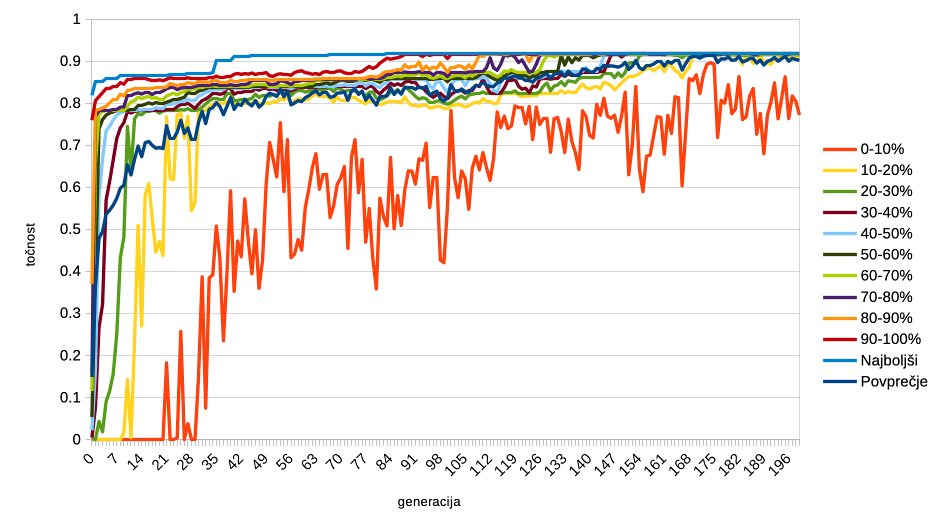
\includegraphics[width=13cm]{shuttle/1/acc}
    \end{center}
    \caption{Graf točnosti populacije najboljšega agenta prvega nabora skozi generacije.}
    \label{fig:statlog_acc_1}
\end{figure}

\begin{figure}[H]
    \begin{center}
        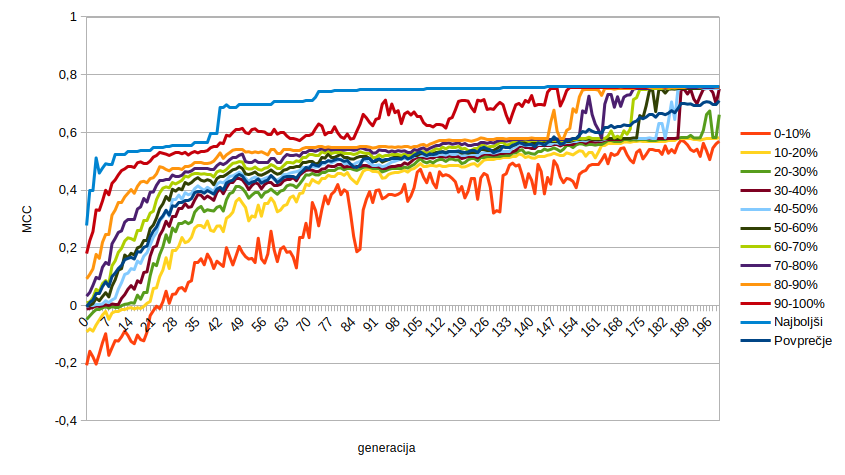
\includegraphics[width=13cm]{shuttle/1/mcc}
    \end{center}
    \caption{Graf MCC populacije najboljšega agenta prvega nabora skozi generacije.}
    \label{fig:statlog_mcc_1}
\end{figure}

\begin{figure}[H]
    \begin{center}
        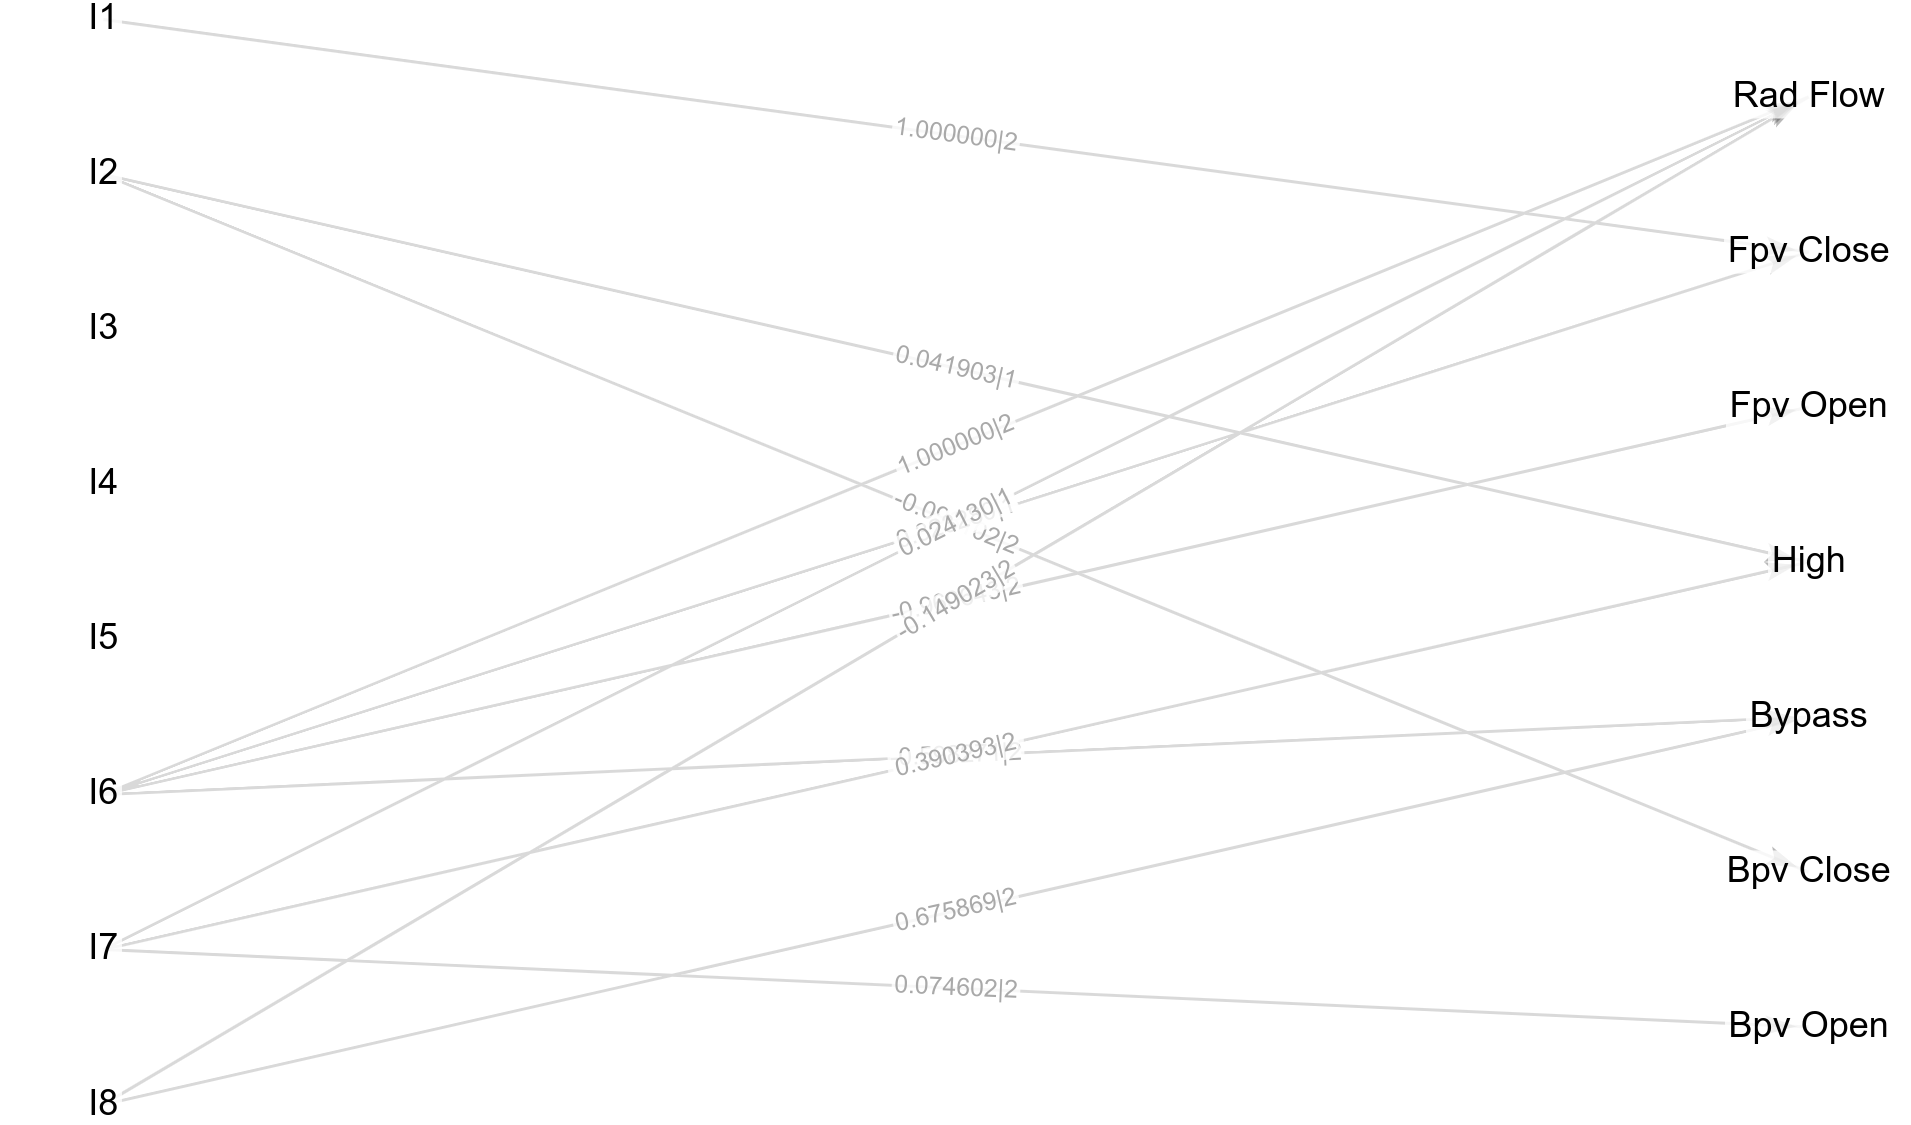
\includegraphics[width=13cm]{shuttle/1/acc_g}
    \end{center}
    \caption{Vizualizacija najbolj točnega agenta prvega nabora. Vsebuje 12 povezav.}
    \label{fig:statlog_acc_1_g}
\end{figure}

\begin{figure}[H]
    \begin{center}
        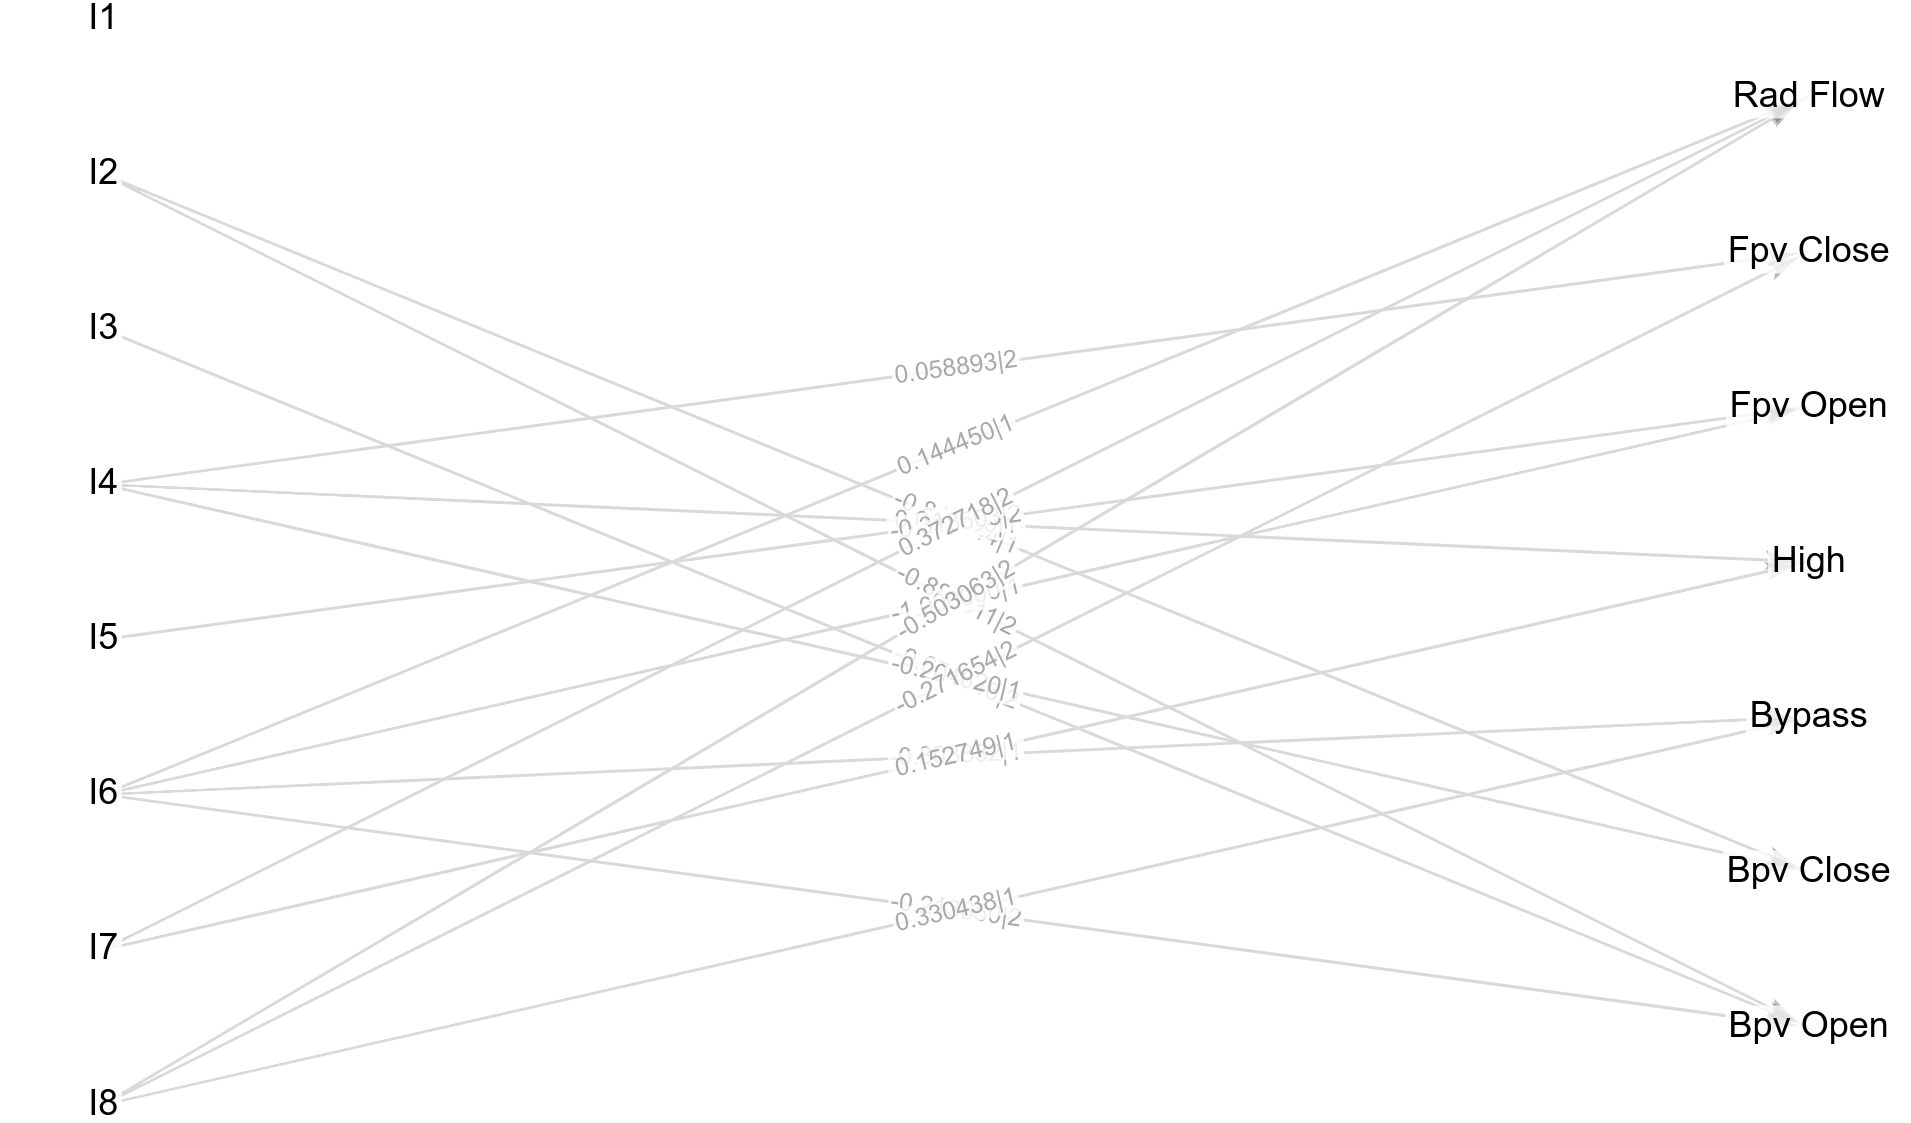
\includegraphics[width=13cm]{shuttle/1/mcc_g}
    \end{center}
    \caption{Vizualizacija agenta z največjim MCC prvega nabora. Vsebuje 1 globoko vozlišče in 21 povezav.}
    \label{fig:statlog_mcc_1_g}
\end{figure}

\subsection{Drugi nabor}\label{subsec:dodatek-statlog-drugi-nabor}
%% 250 20 50 3 true 0.1 125 true -0.00001 250 ACC
\begin{table}[H]
    \begin{center}
        \begin{tabular}{|| c | c c || c c ||}
            \hline
            \multirow{2}{*}{št. zagona} & \multicolumn{2}{c||}{točnost najboljšega agenta} & \multicolumn{2}{c||}{MCC najboljšega agenta} \\ \cline{2-5}
            & učna & testna       & učna & testna           \\
            \hline
            1        & 0\%  & 0\%          & 0    & 0                \\
            \hline
            2        & 0\%  & 0\%          & 0    & 0                \\
            \hline
            3        & 0\%  & 0\%          & 0    & \textbf{0 (0\%)} \\
            \hline
            4        & 0\%  & 0\%          & 0    & 0                \\
            \hline
            5        & 0\%  & \textbf{0\%} & 0    & 0                \\
            \hline
            $\sigma$ & 0    & 0            & 0    & 0                \\
            \hline
        \end{tabular}
    \end{center}
    \caption{Rezultat prvega nabora parametrov.}
    \label{tab:statlog_result_2}
\end{table}

\subsection{Tretji nabor}\label{subsec:dodatek-statlog-tretji-nabor}
%% 350 40 100 4 true 0.1 175 true -0.00001 -0.00001 300 ACC

\section{Random forest}\label{sec:random-forest-test}
\subsection{Iris}\label{subsec:random-forest-iris-test}
\begin{table}[H]
    \centering
    \begin{tabular}{||rcccc||}
        \hline
        razred           & Iris Setosa & Iris Versicolour & Iris Virginica & vsota \\ \hline
        ris Setosa       & 15          & 0                & 0              & 15    \\ \hline
        Iris Versicolour & 0           & 14               & 1              & 15    \\ \hline
        Iris Virginica   & 0           & 1                & 14             & 15    \\ \hline
        vsota            & 15          & 15               & 15             & 45    \\ \hline
    \end{tabular}
    \caption{Matrika zmot pristopa naključnih dreves na množici Iris s točnostjo $94.8\%$ in MKK $0.933$.}
    \label{tab:rforest_iris_cm}
\end{table}

\subsection{Wine}\label{subsec:random-forest-wine-test}
\begin{table}[H]
    \centering
    \begin{tabular}{||rcccc||}
        \hline
        razred  & Class 1 & Class 2 & Class 3 & vsota \\ \hline
        Class 1 & 18      & 0       & 0       & 18    \\ \hline
        Class 2 & 0       & 20      & 1       & 21    \\ \hline
        Class 3 & 0       & 0       & 14      & 14    \\ \hline
        vsota   & 18      & 20      & 15      & 53    \\ \hline
    \end{tabular}
    \caption{Matrika zmot pristopa naključnih dreves na množici Wine s točnostjo $98.1\%$ in MKK $0.972$.}
    \label{tab:rforest_wine_cm}
\end{table}

\subsection{Car}\label{subsec:random-forest-car-test}
\begin{table}[H]
    \centering
    \begin{tabular}{||rccccc||}
        \hline
        razred       & unacceptable & acceptable & good & very good & vsota \\ \hline
        unacceptable & 357          & 6          & 0    & 0         & 363   \\ \hline
        acceptable   & 9            & 105        & 1    & 0         & 115   \\ \hline
        good         & 0            & 8          & 12   & 1         & 21    \\ \hline
        very good    & 0            & 2          & 0    & 17        & 19    \\ \hline
        vsota        & 366          & 121        & 13   & 18        & 518   \\ \hline
    \end{tabular}
    \caption{Matrika zmot pristopa naključnih dreves na množici Car Evaluation s točnostjo $94.8\%$ in MKK $0.885$.}
    \label{tab:rforest_car_cm}
\end{table}

\subsection{Shuttle}\label{subsec:random-forest-shuttle-test}
\begin{table}[H]
    \centering
    \begin{tabular}{||rcccccccc||}
        \hline
        razred    & RF    & FC & FO & High & Bypass & BC & BO & vsota \\ \hline
        Rad Flow  & 11477 & 0  & 1  & 0    & 0      & 0  & 0  & 11478 \\ \hline
        Fpv Close & 0     & 12 & 0  & 1    & 0      & 0  & 0  & 13    \\ \hline
        Fpv Open  & 1     & 0  & 38 & 0    & 0      & 0  & 0  & 39    \\ \hline
        High      & 0     & 0  & 0  & 2155 & 0      & 0  & 0  & 2155  \\ \hline
        Bypass    & 1     & 0  & 0  & 0    & 808    & 0  & 0  & 809   \\ \hline
        Bpv Close & 0     & 0  & 0  & 1    & 0      & 3  & 0  & 4     \\ \hline
        Bpv Open  & 0     & 0  & 1  & 0    & 0      & 0  & 1  & 2     \\ \hline
        vsota     & 11479 & 12 & 40 & 2157 & 808    & 3  & 1  & 14500 \\ \hline
    \end{tabular}
    \caption{Matrika zmot pristopa naključnih dreves na množici Shuttle s točnostjo $100\%$ in MKK $0.999$.}
    \label{tab:rforest_shuttle_cm}
\end{table}

